%% 
%% Copyright 2007-2026 Elsevier Ltd
%% 
%% This file is part of the 'Elsarticle Bundle'.
%% ---------------------------------------------
%% 
%% It may be distributed under the conditions of the LaTeX Project Public
%% License, either version 1.3 of this license or (at your option) any
%% later version.  The latest version of this license is in
%%    http://www.latex-project.org/lppl.txt
%% and version 1.3 or later is part of all distributions of LaTeX
%% version 1999/12/01 or later.
%% 
%% The list of all files belonging to the 'Elsarticle Bundle' is
%% given in the file `manifest.txt'.
%% 
%% Template article for Elsevier's document class `elsarticle'
%% with numbered style bibliographic references
%% SP 2008/03/01
%% $Id: elsarticle-template-num.tex 289 2026-01-09 06:13:01Z rishi $
%%

%% Use the option review to obtain double line spacing
%% \documentclass[authoryear,preprint,review,12pt]{elsarticle}
\documentclass[times, review, 10pt]{elsarticle}

%% Use the options 1p,twocolumn; 3p; 3p,twocolumn; 5p; or 5p,twocolumn
%% for a journal layout:
%% \documentclass[final,1p,times]{elsarticle}
%% \documentclass[final,1p,times,twocolumn]{elsarticle}
%% \documentclass[final,3p,times]{elsarticle}
%% \documentclass[final,3p,times,twocolumn]{elsarticle}
%% \documentclass[final,5p,times]{elsarticle}
%% \documentclass[final,5p,times,twocolumn]{elsarticle}

%% For including figures, graphicx.sty has been loaded in
%% elsarticle.cls. If you prefer to use the old commands
%% please give \usepackage{epsfig}

%% The amssymb package provides various useful mathematical symbols
\usepackage{amssymb}
%% The amsmath package provides various useful equation environments.
\usepackage{amsmath}
%% The amsthm package provides extended theorem environments
%% \usepackage{amsthm}

%% The lineno packages adds line numbers. Start line numbering with
%% \begin{linenumbers}, end it with \end{linenumbers}. Or switch it on
%% for the whole article with \linenumbers.
%% \usepackage{lineno}

\journal{Pattern Recognition}


\usepackage[colorlinks,linkcolor=black,anchorcolor=black,citecolor=black]{hyperref}
\usepackage{graphicx}
\usepackage{epsfig}
\usepackage{amssymb}
\usepackage{mathrsfs}
\usepackage{bm}
\usepackage{color}
\usepackage{amsmath}
\usepackage{mathrsfs}
\usepackage{algorithmic}
\usepackage[linesnumbered,ruled]{algorithm2e}
%\usepackage{algpseudocode}
\renewcommand{\algorithmicrequire}{\textbf{Input:}}
\renewcommand{\algorithmicensure}{\textbf{Output:}}
\usepackage{graphicx}
\usepackage{subfigure}
\usepackage{float}
\usepackage{booktabs}
\usepackage{multirow}

\usepackage{lineno}
\usepackage{ntheorem}

\usepackage{tabularx}
\usepackage[normalem]{ulem}

\biboptions{numbers,sort&compress}



%\usepackage[round,authoryear]{natbib}
% \usepackage{xeCJK}
\usepackage{threeparttable}
\newcommand{\tabincell}[2]{\begin{tabular}{@{}#1@{}}#2\end{tabular}}
\usepackage{caption2}
\renewcommand{\captionlabeldelim}{.}
\renewcommand{\figurename}{Fig.}
%\listoffigures

\newtheorem{theorem}{Theorem}
\newtheorem{definition}{Definition}
\newtheorem{proposition}{Proposition}
\newtheorem{lemma}{Lemma}
\newtheorem{corollary}{Corollary}
\newtheorem*{proof}{Proof:}
\newtheorem{example}{Example}
\newtheorem{property}{Property}

\journal{Pattern Recognition}
\setlength{\subfigcapskip}{-8pt}
\setlength{\abovecaptionskip}{5pt}

% \usepackage[final]{changes}
\usepackage[markup]{changes}

\begin{document}

\begin{frontmatter}

\title{Granular-ball guided Coulomb force for anomaly detection}
\author[adr1]{Shihao Wang}
\ead{wangshihao1@stu.scu.edu.cn}
\author[adr1]{Xinyu Su}
\ead{suxinyu@stu.scu.edu.cn}
\author[adr1]{Dezhong Peng}
\ead{pengdz@scu.edu.cn}
\author[adr1]{Xi Peng}
\ead{pengx.gm@gmail.com}
\author[adr2]{Xiaomin Song}
\ead{songxiaomin@uptcsc.com}
\author[adr1]{Zhong Yuan\corref{cor1}}
\ead{yuanzhong@scu.edu.cn}
\cortext[cor1]{Corresponding author}


\address[adr1]{College of Computer Science, Sichuan University, Chengdu 610065, China}
\address[adr2]{Sichuan National Innovation New Vision UHD Video Technology Co., Ltd, Chengdu 610095, China}


\begin{abstract}

Physics-informed anomaly detection methods have gradually emerged as a topic of interest for scholars. {These methods effectively identify anomalies by constructing anomaly detection models based on the concepts from physics.}
However, they face two main challenges: 
{(1) Existing methods are often restricted to a single perspective, failing to simultaneously capture global structural information and local interaction details, which in turn limits their performance in anomaly detection.} (2) Physics-informed models typically compute pairwise interactions between samples, resulting in limited scalability and high computational costs, while also being susceptible to interference from noise or outliers.
In response to the challenges, a multi-granularity anomaly detection method is proposed integrating local Coulomb force with granular-ball representations.
Specifically, we first employ granular-ball computing to cover samples, enabling an adaptive and efficient multi-granularity representation.
Subsequently, natural neighbor search and fuzzy similarity relationship modeling are performed on the granular-balls, through which global information is extracted.
{To complement this global view, we design the electrified granular-ball (EGB) model, which maps the size of each granular-ball to its charge intensity, enabling an extended Coulomb force formulation that preserves multi-granularity information.}
Building on this model, the local anomaly degree of samples is assessed by computing the anomaly Coulomb force from neighboring EGB.
Finally, anomaly scores are constructed to characterize the anomaly degree of the samples, fusing the information from both perspectives.
Results of experiments on real-world datasets highlight the superiority of the proposed method in detection accuracy over state-of-the-art detection methods, as well as its efficiency and robustness. The source codes are publicly available at https://github.com/Caspar-lab/GBNAD.

\end{abstract}
\begin{keyword}
Anomaly detection; Granular-ball computing; Multi-granularity;  Coulomb force; Natural neighbor
\end{keyword}

\end{frontmatter}

\section{Introduction}

Anomaly detection is a fundamental task in data mining and machine learning,
% \cite{liao2024k}
widely applied in fraud detection \cite{devavarapu2024credit}, network security \cite{sabitha2022fuzzy}, and medical diagnosis \cite{li2023outlier}. 
Depending on the availability of labeled data, anomaly detection methods can be categorized into three main types: supervised \cite{zhang2026deep},
 semi-supervised \cite{lian2025semi},
 and unsupervised
\cite{hu2024multi}.
Among these, unsupervised methods have garnered significant attention due to their applicability in scenarios where labeled data are scarce or unnecessary, particularly for identifying previously unseen anomalous patterns. 
Unsupervised anomaly detection captures the intrinsic structure of data to identify samples that deviate significantly from the normal distribution. This capability renders the approach particularly well-suited for complex environments without labels.

Existing unsupervised anomaly detection methods can generally be categorized into five main types, according to the principles used to identify anomalous samples: density-based methods, statistical-based methods, distance-based methods, clustering-based methods, 
and methods founded on rough set theory (RST).
%\cite{yuan2024dfno}
Besides the above methods, Physics-Informed Machine Learning (PIML)-based methods  
% \cite{yang2025escape}, \cite{bharti2016gravitational}, 
\cite{zhu2022high} emerge as promising unsupervised anomaly detection methods. 
PIML-based methods center on integrating known physical laws into anomaly detection models, enabling models to extract knowledge from data with underlying physical laws. For example, Zhu et al. \cite{zhu2022high} introduced the concepts of anomaly Coulomb force {(ACF)} based on Coulomb's law to identify the anomalies. By fusing data-driven techniques with domain-specific principles, PIML methods offer improved performance and better interpretability compared to conventional purely data-based approaches. 
Despite the growing success of PIML-based methods, many existing algorithms still suffer from high computational complexity, sensitivity to outliers, and single-granularity representation. These limitations hinder the robustness and detection accuracy of PIML models.
{Specifically, existing PIML approaches predominantly operate on a fine-grained, point-wise basis, which leads to quadratic computational costs and increases susceptibility to local noise. There remains a critical gap in mechanisms that can retain the superior performance and physical interpretability of PIML, while simultaneously abstracting data into robust, multi-scale structures for efficient computation.}

{To address this gap, Granular-Ball Computing (GBC) becomes an ideal solution due to its efficient, robust, and interpretable multi-granularity representation \cite{xia2023granular}. Instead of operating on individual samples, GBC processes granular-balls obtained by adaptively covering the original points. While studies have applied GBC to anomaly detection \cite{su2024detecting}, no research has yet combined GBC with PIML models.}
{Consequently, we propose a multi-granularity anomaly detection method fusing local Coulomb force and granular-ball representation (GBNAD). GBNAD directly addresses the aforementioned limitations by shifting the physical interaction mechanism from the sample level to the granular-ball level. This fusion enables the model to shield against outliers through coarse-grained abstraction while significantly reducing computational overhead, thereby achieving a balance between physical interpretability, efficiency, and robustness.}
The proposed method has two essential components, as shown in Fig. \ref{The framework of GBNAD.}.
GBC is first employed to cover the samples and derive the granular-ball set, enabling adaptive and efficient multi-granularity representation.
Subsequently, a natural neighbor search is performed on the set of granular-balls.
Global information is then obtained by leveraging natural neighborhood relationships and granular-ball densities.
{Regarding the second component, the EGB model is introduced, wherein samples are treated as charges in an EGB-induced electric field.} The resultant granular-ball anomaly force exerted on each sample is considered to quantify its local anomaly degree. Vector-based computation preserves both the direction and magnitude information of each attribute, capturing inter-dimensional differences more accurately. 
The contributions of this paper can be summarized as follows.
\begin{enumerate}[\indent(1)]
    \item We proposed a novel anomaly detection framework fusing global and local information with GBC and ACF.
    \item The EGB model is proposed, which improves the computational efficiency and offers greater scalability for the ACF model.
    \item Comprehensive experiments on multiple real-world datasets are conducted, validating the effectiveness, efficiency, and robustness of our approach compared to existing methods.
\end{enumerate}

\begin{figure}[!htb]
    \centering
    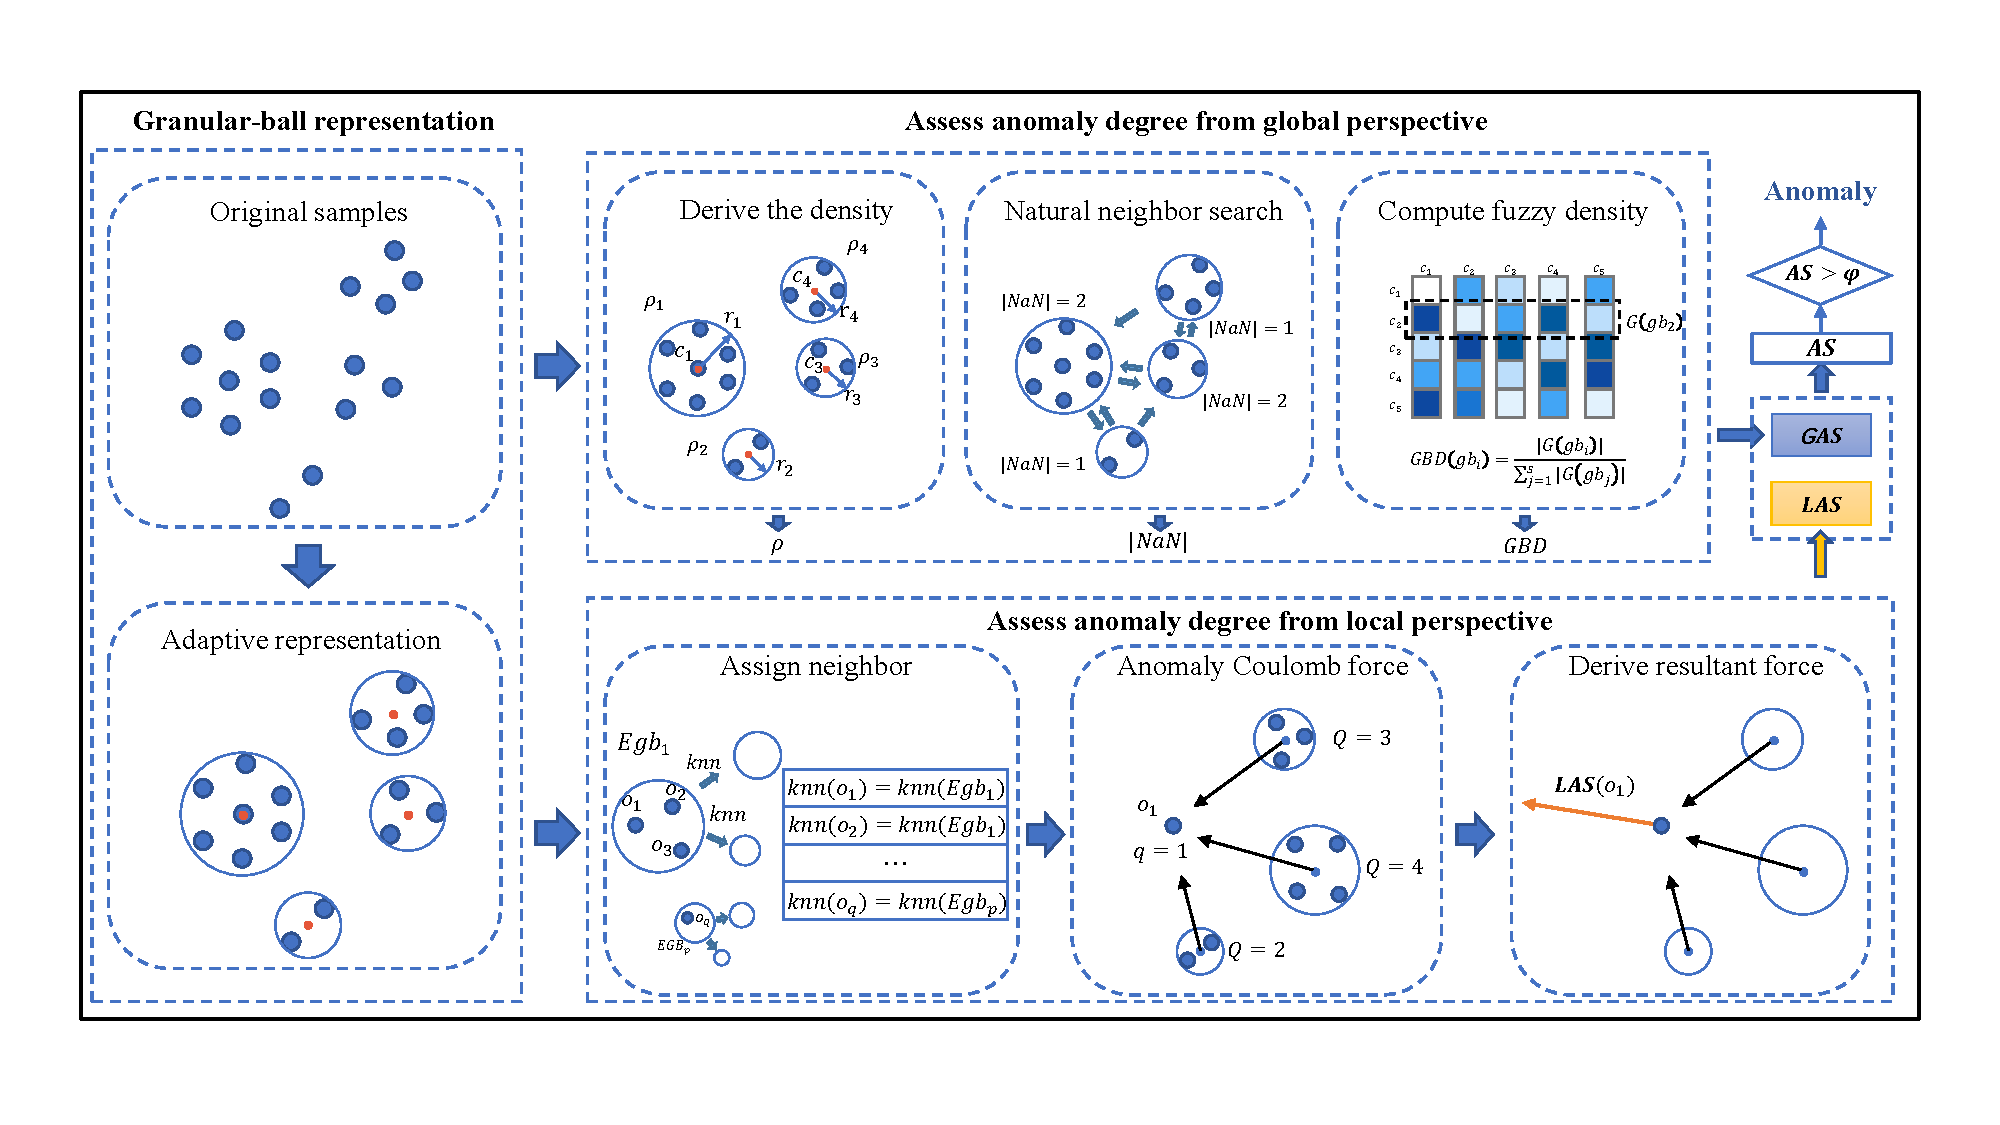
\includegraphics[width=0.95\textwidth]{Framework6.0.pdf}
    \caption{The framework of GBNAD.}
    \label{The framework of GBNAD.}
\end{figure}

The remainder of this paper is organized as follows: Section \ref{Related work} reviews related work on anomaly detection, including PIML-based and GBC-based methods. Section \ref{Preliminaries} presents the theoretical foundation of our approach, followed by the proposed GBNAD framework in Section \ref{The proposed anomaly detection method}. Section \ref{Experiments} provides comprehensive experimental evaluations, and Section \ref{Conclusion} concludes with future research directions.

\section{Related work}
\label{Related work}
In what follows, we first review existing PIML-based anomaly detection methods and their current limitations. Then, we discuss the development and applications of GBC across various tasks, highlighting its potential as a framework to enhance unsupervised anomaly detection.
\subsection{Traditional detection methods and PIML-based detection methods}

{
Among traditional unsupervised anomaly detection methods, a variety of approaches have been extensively studied, including statistical methods, distance-based methods, density-based methods, clustering-based methods, and those grounded in Fuzzy Set Theory (FST). Statistical methods typically fit a model to the majority of the data and identify anomalies as observations that significantly deviate from the assumed distribution \cite{rousseeuw2018anomaly}. Distance-based methods detect outliers by assuming that anomalous samples are located far from most other data points in the feature space \cite{dang2015distance}. Density-based approaches, exemplified by the Local Outlier Factor (LOF) proposed by Breunig et al. \cite{Breunig2000LOF}, identify anomalies by comparing the local density of a point with that of its neighbors. In addition, clustering-based methods group data into clusters and regard samples that deviate significantly from cluster centers as anomalies \cite{degirmenci2022efficient}. Beyond these methods, RST-based approaches have been developed to detect anomalies through multi-granularity computing, and numerous extensions have demonstrated the effectiveness of this paradigm \cite{chen2025label}.
Despite their effectiveness, these methods rely on different underlying assumptions that lead to inherent limitations. Distance-based methods implicitly assume a uniform data distribution and therefore struggle with datasets exhibiting varying local densities, resulting in missed detections of local outliers \cite{li2022robust}. Density-based methods alleviate this issue by modeling local density variations but are still sensitive to neighborhood definition and parameter selection. {Additionally}, both distance- and density-based approaches primarily depend on numerical distance measures, which may limit their applicability to categorical data or complex data structures. Nevertheless, although clustering- and FST- based methods provide a global grouping perspective, they may overlook local or boundary anomalies.
}

While these traditional approaches offer valuable insights, they often rely purely on data-driven learning. In recent years, PIML has emerged as a promising paradigm for integrating physical principles into machine learning algorithms
, and has gained growing attention for its ability to enhance model generalization and interpretability.
Within the context of anomaly detection, several PIML-based methods have been proposed. 
For example, Xie et al. \cite{xie2020local} proposed a local gravitation-based method. They modeled each data point as a mass-bearing object influenced by a local resultant force exerted by its neighbors. Points experiencing greater force variation are more likely to lie on decision boundaries. Zhu et al. \cite{zhu2022high} introduced the concepts of ACF and proposed the NHOD algorithm to capture inter-dimensional disparities and alleviate the curse of dimensionality. {Furthermore}, Liu et al. \cite{liu2025outlier} employed potential energy, a fundamental physics principle, to represent local densities and neighbor distributions. {In addition}, Yang et al. \cite{yang2025escape} proposed a novel, escape velocity-based adaptive outlier detection algorithm, which estimates the escape velocity for each sample and identifies outliers by tracking variations of these velocities. 

However, existing PIML-based methods still suffer from two critical limitations. 
{First, most approaches perform anomaly detection from a single local perspective or at a single granularity. As a result, they struggle to jointly capture global structural information and local anomalous patterns. At the same time, this leads to inefficient computation and increased sensitivity to outliers.
Second, many existing methods rely on fixed processing units. This limits their ability to integrate multi-scale structural information and constrains the flexible extension of embedded physical models.}

\subsection{Granular-ball computing}

GBC was originally developed to improve the efficiency of supervised learning by simulating the human brain’s coarse-to-fine recognition mechanism \cite{xia2019granular}. This approach employs granular-balls of varying granularity to cover data samples, thereby achieving an adaptive and efficient multi-granularity representation. As a novel granular computing method, GBC has demonstrated notable performance improvements across diverse domains.

Among the various applications of GBC, clustering is one of the most widely explored domains.
% \cite{xie2024adaptive}
For instance, Xia et al. proposed a novel clustering algorithm called GBCT \cite{xia2025gbct}, which aims to address the low efficiency, limited generalization, and insufficient robustness of traditional clustering methods. 
{Furthermore, GBC is increasingly being adapted for classification. Xie et al. \cite{xie2025approximate} proposed a GB-based approximate borderline sampling method, solving the issues of class boundary blurring and noise caused by traditional GB overlaps. In the field of multi-view learning, Wang et al. \cite{wang2025capturing} combined granular-ball topology construction and collaborative matrices to propose a multi-view graph convolutional network, addressing the limitation of existing view fusion modes that overlook local information within individual views.}


GBC has also been employed in outlier detection. Recent studies have introduced multi-granularity Granular-Balls (GBs) to replace individual data points for coarse-grained outlier detection. By analyzing point density, overlap, and neighborhood changes of GBs, Bai et al. \cite{bai2023granular} proposed a robust and adaptive coarse-grained detection method that improves both efficiency and noise resilience compared to traditional methods. Su et al. \cite{su2024detecting} presented an unsupervised anomaly detection method, which utilizes the fuzzy rough sets to mine the uncertainty information. Besides, Wang et al. \cite{wang2025granular} constructed a GB-based state transfer matrix to integrate GBC and Random walk.

{In addition}, recent works have significantly strengthened the theoretical foundation of GBC in uncertainty modeling and rough sets. For instance, Yang et al. constructed a three-way decision model using fuzzy granular-ball rough sets based on uncertainty invariance \cite{yang2025constructing}, and proposed a cost-sensitive three-way granular-ball generation method (CS3W-GBG) \cite{yang2025cs3w}. These studies provide a solid theoretical basis for the multi-granularity representations and uncertainty handling mechanisms utilized in this manuscript.

{Despite these achievements, applications of GBC in anomaly detection remain limited compared to its widespread use in clustering, compounded by the limited interpretability of existing GBC-based methods.} Therefore, it is worth exploring to fusing the advantages of GBC and PIML for unsupervised anomaly detection.


\section{Preliminaries}
\label{Preliminaries}
This section introduces the granular-ball theory and ACF theory to provide a theoretical foundation for our proposed method. These concepts help illustrate the underlying principles and mechanisms that drive our approach to anomaly detection.

\subsection{Granular-ball representation}
\label{GB representation}
This subsection introduces the process of covering the dataset with granular-balls.
Dataset is given as $\boldsymbol{X} =\left[\boldsymbol{x_1} ; \boldsymbol{x_2} ; \ldots ; \boldsymbol{x_n} \right] \in \mathbb{R}^{n \times m}$, where $n$ is the number of samples and $\boldsymbol{x_i}=\left[a_1, a_2, \cdots, a_m\right] \in \boldsymbol{X}$ is
denoted by a $m$-dimensional vector. Inspired by the large-scale priority nature of human cognition, Xia et al. \cite{xia2019granular} proposed the GBC model to make the inputs scalable and efficient. 

\begin{definition}
Given a granular-ball set $GBS=\left\{{gb}_1,{gb}_2, \ldots, {gb}_{{s}}\right\}$.
The $k$-th granular-ball $gb_k$ of $GBS$ is only defined by two parameters: radius $r_k$ and center $\boldsymbol{c_k}$, which are defined as
\begin{equation}
\boldsymbol{c_k}=\frac{1}{|gb_k|} \sum_{i=1}^{|g b_k|} \boldsymbol{x_i}, \boldsymbol{x_i} \in g b_k,
\label{Eq:centers}
\end{equation}

\begin{equation}
r_k=\max \left\|\boldsymbol{x_i}-\boldsymbol{c_k}\right\|, \boldsymbol{x_i} \in g b_k.
\label{Eq:radius}
\end{equation}
\end{definition}


One of the key issues in GBC is how to formulate the criteria for granular-ball splitting. To obtain a set of high-quality granular-balls, we adopt the granular-ball splitting criterion proposed in \cite{xie2023efficient}. Initially, 2-means clustering is applied to all input samples to obtain two initial granular-balls. Subsequent distribution analysis of the samples within the balls is required to assess whether further subdivision is necessary.
\begin{definition}
The distribution measurement $QM$ of $gb_k$ is evaluated according to the quantity and the dispersion extent of the samples in the ball, which is defined as
\begin{equation}
QM_k=\frac{\sum\limits_{i=1}^{|g b_k|}\left\|\boldsymbol{x_i}-\boldsymbol{c_k}\right\|}{\sqrt{|gb_k|}},
\end{equation}
\end{definition}
where $|gb|$ is the number of samples within $gb_k$. 

\begin{definition}
Then the weighted distribution measurement is used to determine whether the granular-ball needs further splitting, which is defined as
\begin{equation}
{
SM_{split}(gb_k)=\frac{\left|gb_k(1)\right|}{|gb_k|} QM_1+\frac{\left|gb_k(2)\right|}{|gb_k|} QM_2,}
\label{eq:split critirion}
\end{equation}
\end{definition}
{where $gb_k(1)$ and $gb_k(2)$ denote the sub-balls of $gb_k$.} Further splitting is necessary if $QM$ of $gb_k$ is lower than the $SM_{split}$ of it. When the number of granular-balls at the end of the $t$-th iteration is the same as that at the end of the $(t-1)$-th iteration, the granular-ball generation process is finished. 
{It is important to note that the generation strategy follows the strategy in \cite{xie2023efficient}, and the time complexity of this granular-ball generation phase is $O(n \log n)$.}


\subsection{Fuzzy set theory}
{
Fuzzy set theory is a mathematical framework that models uncertainty by allowing elements to belong to a set with continuous degrees of membership rather than crisp binary assignments \cite{chen2025label}.
Under the granular computing paradigm, a fuzzy information granule can be regarded as a fuzzy set equipped with explicit structural and semantic meaning, enabling uncertainty-aware and multi-granularity data representation.
}

{
Given dataset $\boldsymbol{X}$, the granular-ball set $GBS$ can be derived as \ref{GB representation}. Subsequently, the data can be represented as a 2-tuple $S = <GBS, A>$, where $GBS=\left\{{gb}_1,{gb}_2, \ldots, {gb}_{{s}}\right\}$ is a non-empty finite set of granular-balls and $A$ is a non-empty finite set of conditional attributes.
\begin{definition}
    Given $\mathcal{A} \subseteq A$, the fuzzy relation w.r.t. $\mathcal{A}$ on $GBS$ is denoted as
    \begin{equation}
        R_{\mathcal{A}}: GBS\times GBS \rightarrow [0,1].
    \end{equation}
\end{definition}
}

{
For $\forall gb_{i}, gb_{j} \in GBS$, if 1) $R_{\mathcal{A}}(gb_{i},gb_{i})=1$ (reflexivity) and 2) $R_{\mathcal{A}}(gb_{i},gb_{j})=R_{\mathcal{A}}(gb_{j},gb_{i})$ (symmetry) are satisfied, then $R_{\mathcal{A}}$ is said to be a fuzzy similarity relation. 
Subsequently, the fuzzy information granules can be induced by $R_{\mathcal{A}}$ \cite{wang2025granular}. 
\begin{definition}
    For $\forall gb_{i} \in GBS$, the fuzzy information granule induced by $R_{\mathcal{A}}$ is defined as
\begin{equation}
    G(gb_{i}) = \{R_{\mathcal{A}}(gb_{0},gb_{i}), R_{\mathcal{A}}(gb_{1},gb_{i}),\cdots,R_{\mathcal{A}}(gb_{s},gb_{i})\}.
\end{equation}
\end{definition}
}

{
As the information granule is a collective of elements aggregated based on similarity, the capacity of it can reflect the overall similarity to $GBS$, which is calculated by
\begin{equation}
    |G(gb_{i})| = \sum_{j=1}^{s} R_{\mathcal{A}}(gb_{j},gb_{i})
\end{equation}
}

\subsection{Anomaly Coulomb force}
\label{Anomaly Coulomb force}


Coulomb's law is a physical law discovered by the French physicist Charles Coulomb in 1785 \cite{zhu2022high}. Coulomb proved that there is an interaction force between two charged samples, and the quantitative relationship can be expressed by an equation. 
\begin{definition}
In a vacuum, Coulomb's law can be expressed as
\begin{equation}
F=\frac{q q^{\prime}}{4 \pi \epsilon_0 d^2},
\end{equation}
\end{definition}
where $F$ is the force, $q$ and $q'$ stand for the samples, as well as the amount of charges, $d$ is the distance between them, and $\epsilon_0$ is the vacuum permittivity. 
\begin{definition}
In addition, in order to obtain the direction of the force $F$ of $q^{\prime}$ acting on $q$, we use the vector form of Coulomb's law
\begin{equation}
\label{columb formulation}
{\boldsymbol{F}(\boldsymbol{x_{i}},\boldsymbol{x_{j}})}=\frac{1}{4 \pi \epsilon_0} \frac{q q^{\prime}(\boldsymbol{x_{i}}-\boldsymbol{{x_j}})}{\left\|\boldsymbol{x_i}-\boldsymbol{x_j}\right\|^m}=k_c \frac{q q^{\prime}\boldsymbol{v}}{\left\|\boldsymbol{x_i}-\boldsymbol{{x_j}}\right\|^{m-1}},
\end{equation}
\end{definition}
{
where $\boldsymbol{x_i}$ and ${\boldsymbol{x_j}}$ are the positions of the two samples respectively, $k_c$ denotes the Coulomb constant, $\boldsymbol{v}$ denotes the unit vector from $\boldsymbol{{x_i}}$ to $\boldsymbol{x_j}$, $m$ is the feature dimension of the dataset and  $\left\|\boldsymbol{x_i}-\boldsymbol{{x_j}}\right\|$ represents the euclidean distance between $\boldsymbol{x_i}$ and $\boldsymbol{{x_j}}$.}


According to Zhu et al. \cite{zhu2022high}, the Coulomb force vector encompasses both distance and directional information, allowing it to characterize the similarities and differences among samples more comprehensively. 

\begin{definition}
Furthermore, in order to allow the anomaly electric field strength to be elevated as the distance between samples increases, the anomaly electric field strength \cite{zhu2022high} is defined as 
\begin{equation}
E(\boldsymbol{x_{i}},\boldsymbol{x_{j}})=k_c q_{j}\left\|\boldsymbol{x_i}-\boldsymbol{x_j}\right\|^{m-1},
\end{equation}
\end{definition}
{where $E$ denotes the electric field intensity at the position of $\boldsymbol{x_{i}}$ in the electric field with $\boldsymbol{x_{j}}$ as a field source charge.}
Building on the above definitions, the sample $\boldsymbol{x}_{i}$ in $\boldsymbol{X}$ can be regarded as a charge in a $m$-dimension anomaly electric field $E$ induced by other samples. Furthermore, the resultant force acting on $\boldsymbol{x}_{i}$ can be calculated according to the field intensity, which reflects the degree of deviation from the surrounding samples.
% 进一步地，由场强可以计算得到xi所受库仑合力的大小，而库仑合力则反映了与周围样本的偏离程度。

\begin{definition}
{
The resultant force ${\boldsymbol{F}_{sum}(\boldsymbol{x_i})}$ represents the degree of difference between $\boldsymbol{x_i}$ and nearby samples, which consists of multiple anomaly forces and is calculated by
\begin{equation}
{\boldsymbol{F}_{sum}(\boldsymbol{x_{i}})}=\sum_{\boldsymbol{{x_j}} \in \boldsymbol{X} / \boldsymbol{x_i}} E(\boldsymbol{x_i}, \boldsymbol{x_j})q_{i}\boldsymbol{v}(\boldsymbol{x_i}, \boldsymbol{x_j}),
\end{equation}}
\end{definition}
where $q_{i}$ denotes the charge of $\boldsymbol{x_{i}}$, and $\boldsymbol{v}(\boldsymbol{x_i}, \boldsymbol{x_j})$ denotes the unit vector pointing from $\boldsymbol{x_j}$ to $\boldsymbol{x_i}$.
If ${\boldsymbol{F}_{sum}(\boldsymbol{x_i})}$ exhibits a significant Coulomb force component in some dimension, it indicates that $\boldsymbol{x_i}$ deviates markedly from others in that dimension and may be an anomaly.

Due to the forces of different directions, the resultant Coulomb force on the sample at the center of a uniformly arranged group is small. In particular, the resultant force on the center electrons is zero when the surrounding electron arrangement satisfies strict symmetry, as shown in Fig. \ref{Diagram of electric field strength}. Two electrons of the same charge are represented as blue dots, and the distribution of the electric field is roughly depicted by red curves with arrows representing the direction. The density of the electric field lines represents the strength of the electric field, the denser the greater the field strength. {As can be seen from the figure, the electric field lines at the midpoint of the two charges are the sparsest, indicating that the charges at that location will be under a resultant force of zero.}

\begin{figure}[!htb]
    \centering
    \subfigure[Diagram of electric field strength]{
        \label{Diagram of electric field strength}
        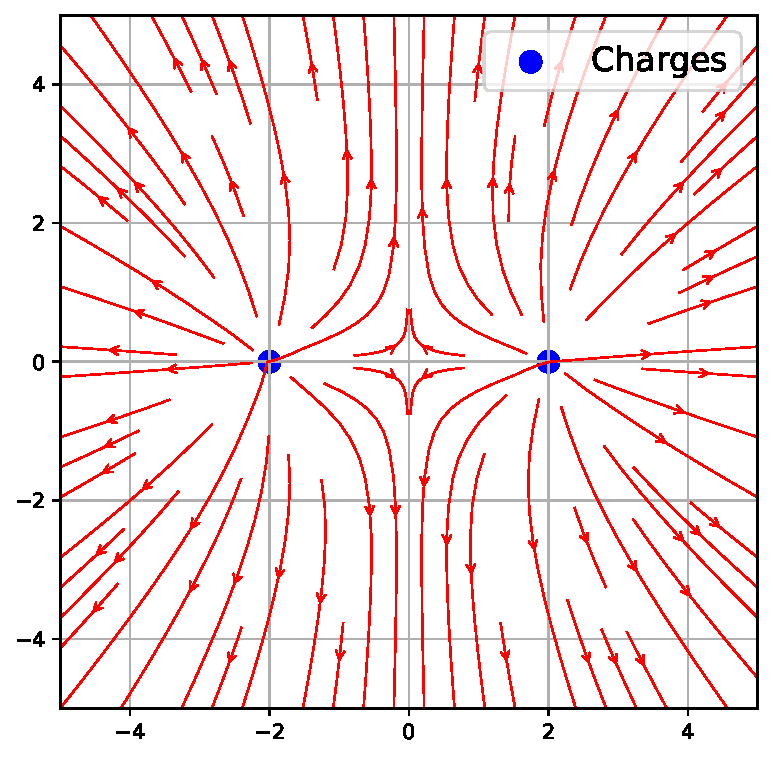
\includegraphics[width=0.33\textwidth]{Electric_field.pdf}}
    \hspace{-0.1in}
    \subfigure[Sparser distribution]{
        \label{Coulomb force simulation(1)} %% label for first subfigure
        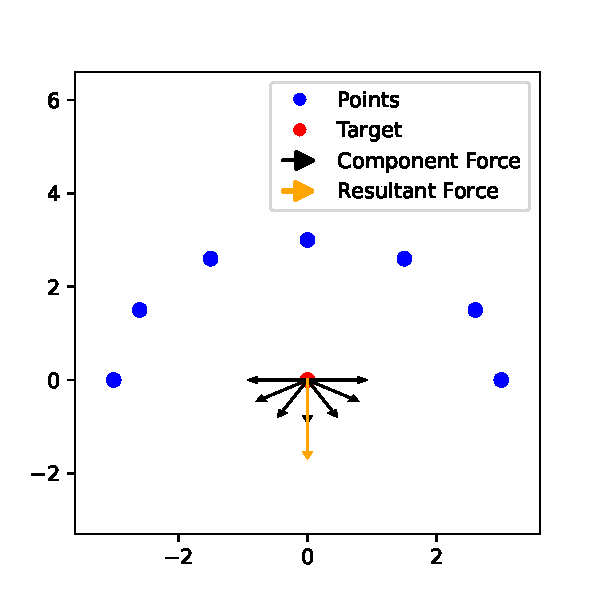
\includegraphics[width=0.33\textwidth]{plot_0_180.pdf}}
    \hspace{-0.1in}
    \subfigure[Denser distribution]{
        \label{Coulomb force simulation(2)} %% label for first subfigure
        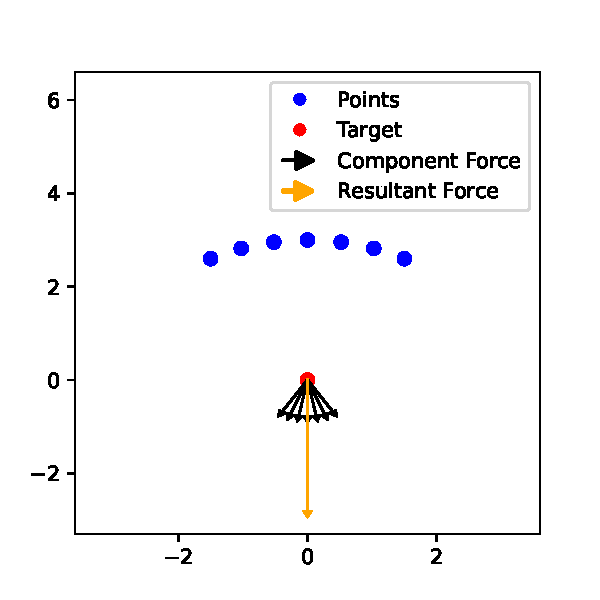
\includegraphics[width=0.33\textwidth]{plot_30_120.pdf}}
    \caption{Illustration of anomaly electric field and anomaly force.}
    \label{Example of resultant anomaly Coulomb force} %% label for eTIRODe figure
\end{figure}

Moreover, as shown in Fig. \ref{Example of resultant anomaly Coulomb force}, it is evident that the resultant ACF effectively reflects anomaly degrees. In Fig. \ref{Coulomb force simulation(1)}, the blue points are more widely scattered, so the center point experiences forces in multiple directions that partially cancel each other out. Consequently, the resultant force on the center point is smaller than that of the center point in Fig. \ref{Coulomb force simulation(2)}. 
Even though the distance from the center to each edge point is the same in both figures, the difference in how those points are distributed leads to notably different resultant forces on the center. Calculating the resultant Coulomb force rather than relying only on distances provides a more interpretable view of anomaly assessment.


\section{The proposed anomaly detection method}
\label{The proposed anomaly detection method}

This section introduces the core theoretical framework of the proposed anomaly detection method GBNAD, which integrates GBC with the ACF concept. Furthermore, a theoretical time complexity analysis is provided to demonstrate the computational efficiency of the algorithm.

\subsection{Global anomaly detection based on granular-balls}

Granular-balls are constructed based on the data distribution, thereby encapsulating implicit structural information. As illustrated in Fig. \ref{fig:natural neighbor}, granular-balls are represented by circles with distinct colors. Red dots denote the centers of granular-balls, while blue dots represent the original input samples. It can be observed that granular-balls located in data-dense regions are tighter, characterized by a larger number of contained samples and a smaller radius. Based on this observation, the density of a granular-ball can serve as an effective metric to assess the anomaly degree of the samples within it.

\begin{figure}[!htb]
	\centering
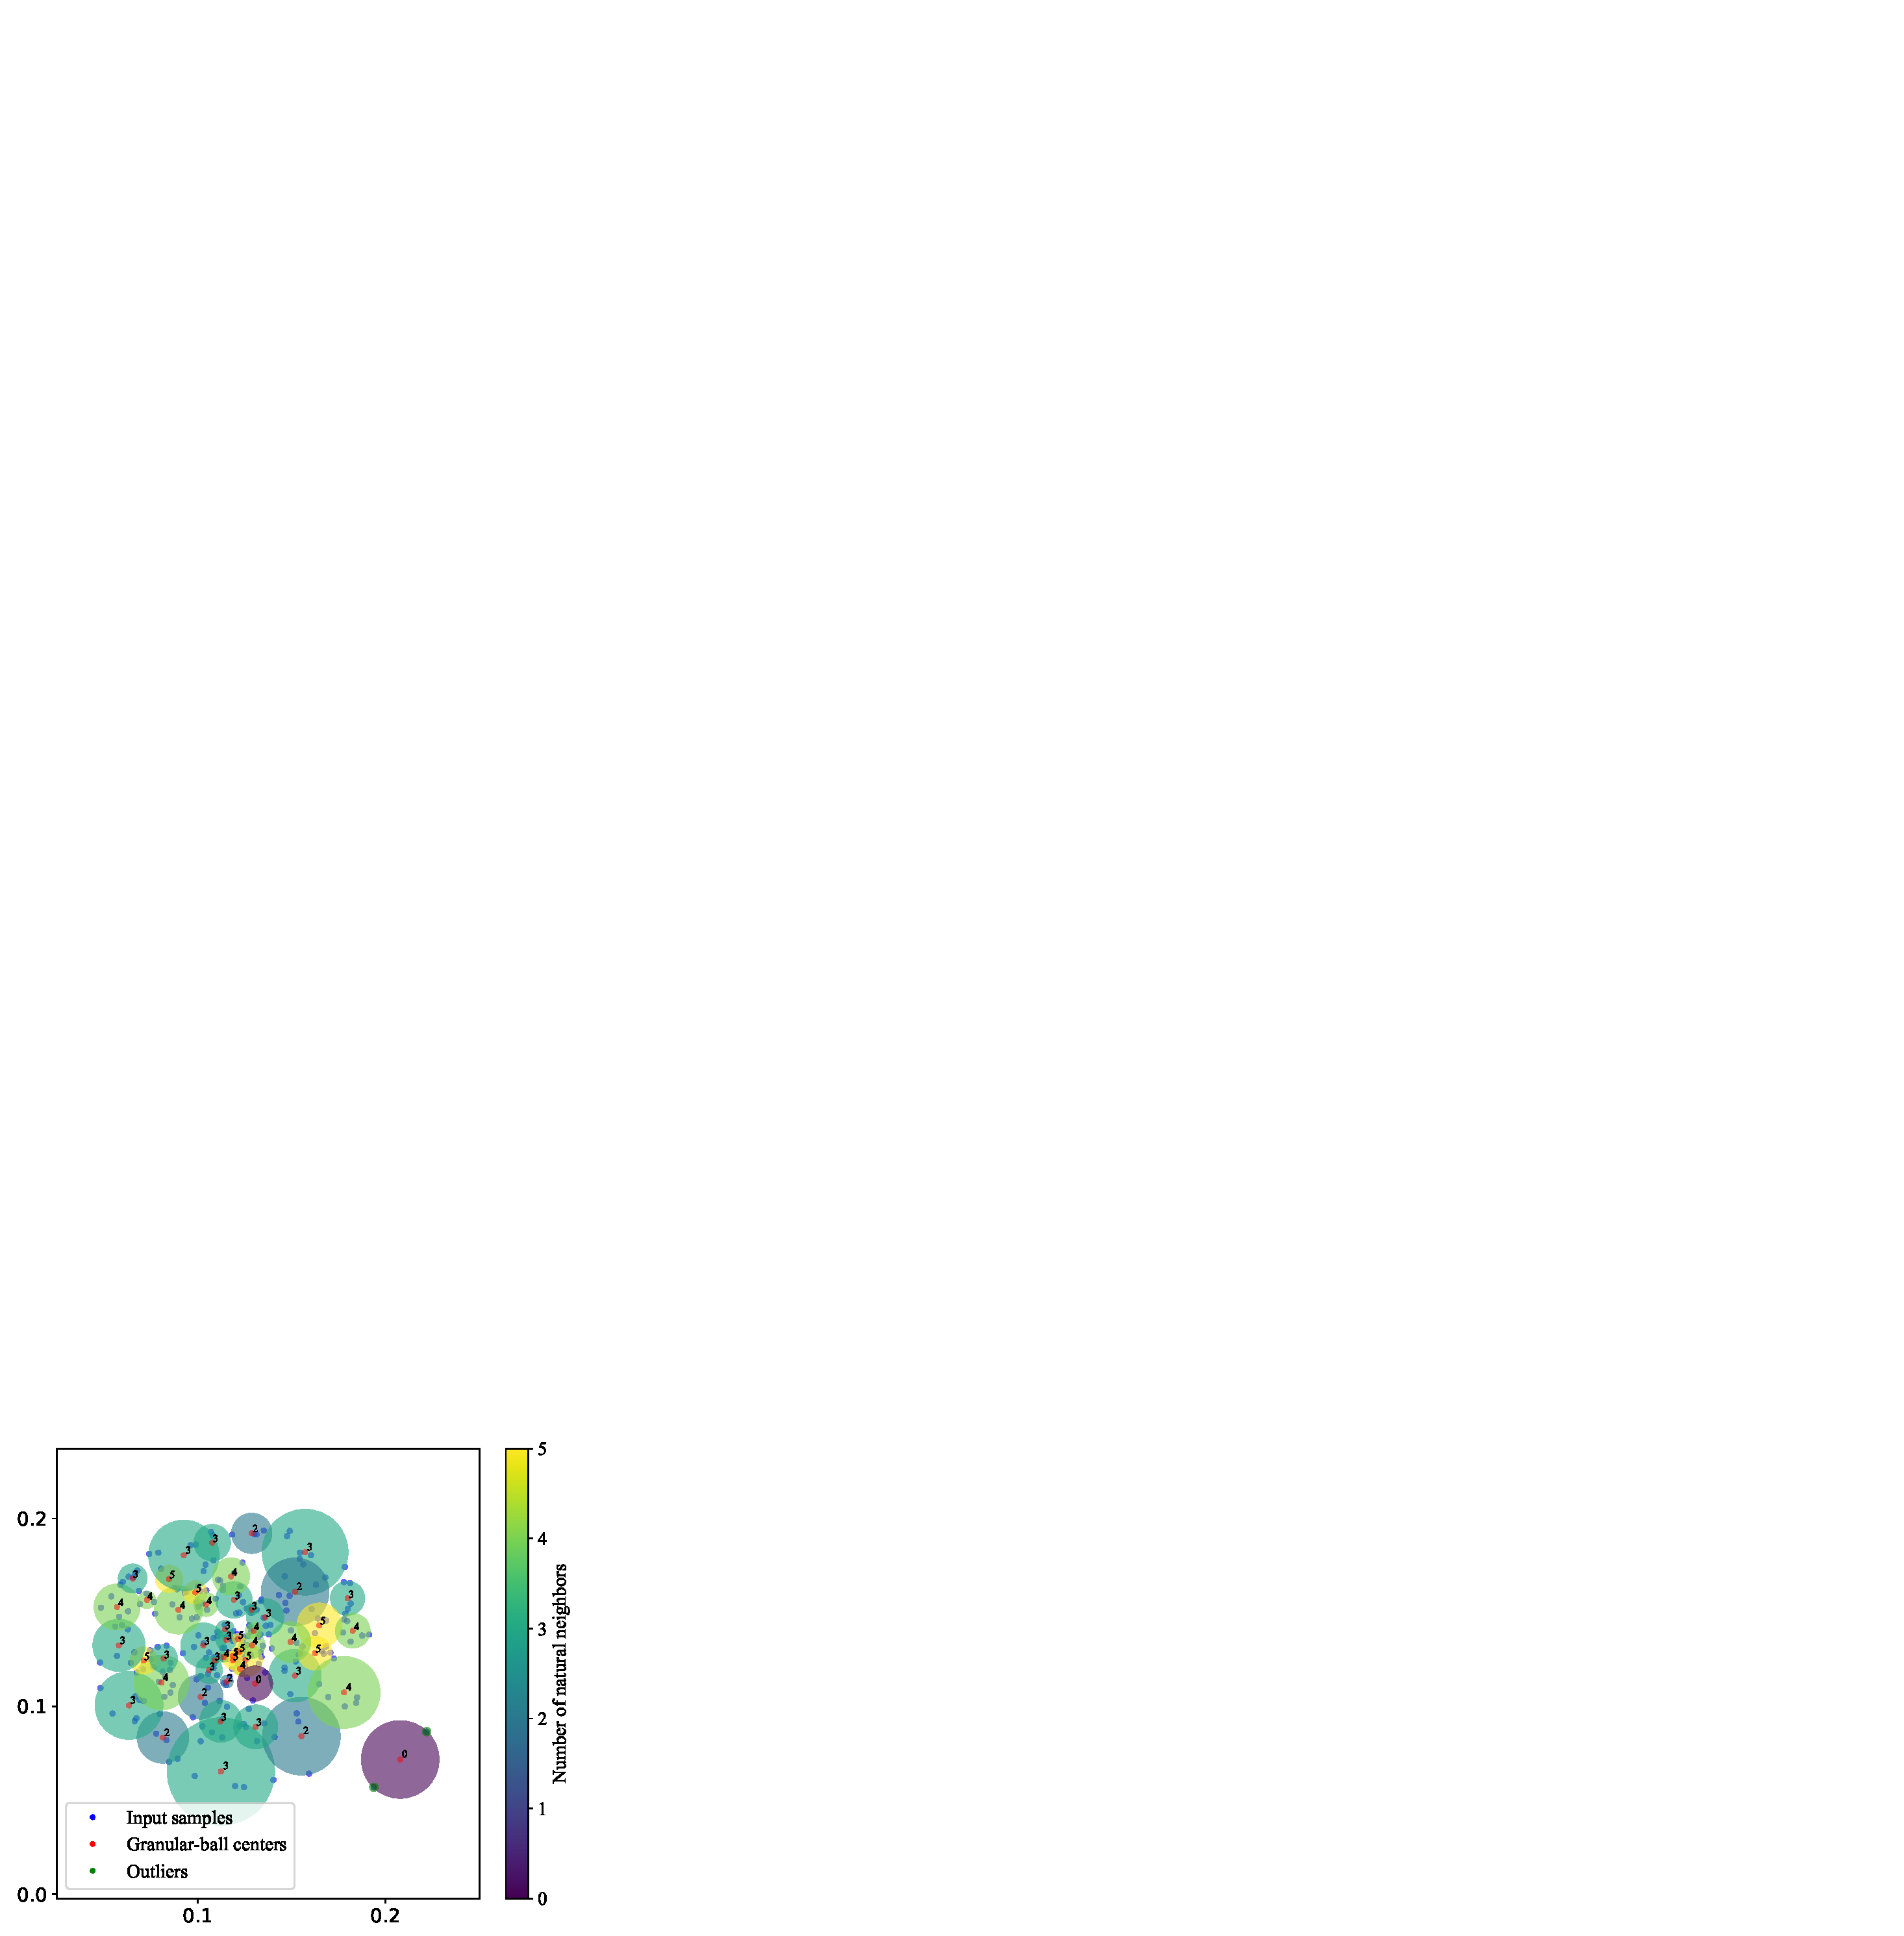
\includegraphics[width=0.5\linewidth]{Granular-Balls Natural Neighbor.pdf}
	\caption{{Visualization of granular-balls and their natural neighbors.}}
    \label{fig:natural neighbor}
\end{figure}

\begin{definition}
The density of the $k$-th granular-ball incorporates both the cardinality and the radius of $gb_k$, which is defined as
\begin{equation}
    \rho_k=\frac{|gb_k|}{r_k},
    \label{eq:rho}
\end{equation}
where $|gb_k|$ represents the number of samples contained in the $k$-th granular-ball, and $r_k$ is its radius.
\end{definition}

Although granular-ball density captures global distribution characteristics from a statistical perspective, relying on this single metric is insufficient for a comprehensive global anomaly assessment. Accordingly, we employ granular-ball-based fuzzy information granules and natural neighborhood structures to characterize global anomaly patterns from complementary perspectives.
First, to construct fuzzy information granules, we define the distance and fuzzy relation between granular-balls.

{
\begin{definition}
    For any two granular-balls $gb_{i}, gb_{j} \in GBS$ with their respective centers denoted as $c_i$ and $c_j$, and an attribute subset $\mathcal{A} \subseteq A$, the distance between $gb_{i}$ and $gb_{j}$ is calculated as
    \begin{equation}
        D_{\mathcal{A}}(gb_{i}, gb_{j}) = \sqrt{\sum_{a\in\mathcal{A}}(c_{i}^{a}-c_{j}^{a})^2},
    \end{equation}
    where $c_i^a$ and $c_j^a$ represent the values of the centers $c_i$ and $c_j$ on attribute $a$, respectively.
\end{definition}
}

\begin{definition}
    Based on the distance metric, the fuzzy relation $R_{\mathcal{A}}$ between $gb_{i}$ and $gb_{j}$ on attribute subset $\mathcal{A}$ is defined as:
    \begin{equation}
        R_{\mathcal{A}}(gb_{i}, gb_{j}) = \exp\!\left(-\frac{D_{\mathcal{A}}(gb_{i}, gb_{j})^2}{2\sigma^2}\right),
    \end{equation}
    {where $\sigma>0$ is a scaling parameter controlling the decay rate of fuzzy similarity. This formulation maps the distance into a continuous similarity measure within $(0,1]$, and we empirically set $\sigma = 1$ as the default value to ensure a stable similarity mapping.}
\end{definition}

In existing Fuzzy Set Theory (FST)-based anomaly detection studies \cite{su2024detecting}, a fuzzy radius is often introduced to emphasize local neighborhood information. In contrast, the fuzzy similarity relation in this work is constructed to capture coarse-grained global structural information; thus, no fuzzy radius is imposed. 
\begin{definition}
Based on the fuzzy relation $R_{\mathcal{A}}$, the fuzzy density of a granular-ball is defined as
    \begin{equation}
    GBD(gb_i) = \frac{|G(gb_i)|}{\sum_{j=1}^{s}|G(gb_j)|},
    \label{eq:fuzzy density}
\end{equation}
where $|G(gb_i)| = \sum_{j=1}^{s} R_{\mathcal{A}}(gb_i, gb_j)$ denotes the information granule cardinality of $gb_i$. A granular-ball exhibits a high degree of global anomaly when its $GBD$ is small, indicating low global similarity with other granular-balls and topological isolation.
\end{definition}

To further capture global structural information induced by the data distribution, we introduce the natural neighbor relationship among granular-balls. Unlike $k$ Nearest Neighbors (kNN) \cite{stevens1951handbook} or Reverse $k$ Nearest Neighbors (RkNN) \cite{korn2000influence}, Natural Nearest Neighbor (NaN) \cite{zhu2016natural} avoids the manual selection of the parameter $k$. The concept is inspired by the stability of neighbor structures during an iterative search process.

\begin{definition}
Let $kNN_\lambda(\boldsymbol{x})$ denote the neighborhood of $\boldsymbol{x}$ when the search process reaches a stable state after $\lambda$ iterations. The natural neighbor relationship is defined as \cite{zhu2016natural}
\begin{equation}
    \boldsymbol{x}_j \in NaN(\boldsymbol{x}_i) \Leftrightarrow \left( \boldsymbol{x}_i \in kNN_\lambda(\boldsymbol{x}_j) \right) \land \left( \boldsymbol{x}_j \in kNN_\lambda(\boldsymbol{x}_i) \right).
\end{equation}
\end{definition}

Accordingly, we extend this concept to the granular-ball level.
\begin{definition}
    The natural neighbor relationship between granular-balls is defined as
    \begin{equation}
        gb_j \in NaN(gb_i) \Leftrightarrow \left( gb_i \in kNN_\lambda(gb_j) \right) \land \left( gb_j \in kNN_\lambda(gb_i) \right).
    \end{equation}
\end{definition}

The procedure for identifying natural neighbors of granular-balls is outlined in Algorithm \ref{GBNAD-alg2}. Xie et al. \cite{xie2024adaptive} observed that samples in data-dense regions tend to possess more natural neighbors. To verify whether this property holds for granular-balls, we visualized the natural neighbor counts in Fig. \ref{fig:natural neighbor}. Granular-balls in denser regions have more natural neighbors (lighter color), while those in sparse regions have fewer (darker color). This confirms that the number of natural neighbors is a valid indicator of global density.
\begin{algorithm}[!ht]
		\caption{Granular-ball Natural Neighbor Search}
            \label{GBNAD-alg2}
		\LinesNumbered
		\KwIn{Granular-ball set $GBS$;}
		\KwOut{Natural Neighbor set $NaN$, $kNN$ graph;}
            Initialize $NaN_{Edge} \leftarrow \emptyset$\;
            Construct a $k$-d tree $T$ from the centers of $GBS$\;
            Initialize $\lambda = 1$, $Flag = False$\;
            \While{Flag == False}{
            \For{\textbf{each} $gb \in GBS$}{
                $knn_\lambda(gb) \leftarrow findkNN(gb,\lambda,T)$\;
                $kNN_\lambda(gb) \leftarrow kNN_\lambda(gb)\cup\{knn_\lambda(gb)\}$\;
            }
            \For{\textbf{each} $gb_i \in GBS$}{
                \For{\textbf{each} $gb_j \in kNN_\lambda(gb_i)$}{
                \If{$gb_i \in kNN_\lambda(gb_j)$ \textbf{and} $gb_j \in kNN_\lambda(gb_i)$ \textbf{and} $\{gb_i,gb_j\}\notin NaN_{Edge}$}{
                $NaN_{Edge} \leftarrow NaN_{Edge}\cup\{gb_i,gb_j\}$\;
                $NaN\_Num(gb_i) \leftarrow NaN\_Num(gb_i)+1$\;
                $NaN\_Num(gb_j) \leftarrow NaN\_Num(gb_j)+1$\;
            }
            }
            }
            \For{\textbf{each} $gb \in GBS$}{
            \If{$NaN\_Num(gb) \neq 0$}{
                $Flag \leftarrow True$\;
            }
            }
            $\lambda \leftarrow \lambda+1$\;
            }
            \Return {$NaN, kNN$}.
\end{algorithm}

Based on the analysis above, the global anomaly degree is jointly evaluated using three complementary metrics: information granule cardinality, granular-ball density, and the number of natural neighbors.

\begin{definition}
The Global Anomaly Score ($GAS$) for a sample $\boldsymbol{x} \in gb_i$ is defined as
\begin{equation}
    GAS(\boldsymbol{x}) = {\frac{\sum_{j=1}^{s}|G(gb_j)|}{\sqrt{\rho_{i} \cdot \max(1, |NaN(gb_i)|)} \cdot |G(gb_i)|  }},
    \label{eq:coarse-grained degree}
\end{equation}
where $\rho_i$ is the density of $gb_i$, and $|NaN(gb_i)|$ is the number of natural neighbors. The term $\max(1, |NaN(gb_i)|)$ ensures numerical stability for isolated granular-balls.
\end{definition}

\subsection{Local anomaly detection based on EGB and Anomaly Force}

While the global anomaly score provides structural insights, local anomaly detection remains essential for identifying boundary outliers and local density deviations. This section introduces the Electrified Granular-Ball (EGB) model and the Anomaly Coulomb Force (ACF) to evaluate local anomalies.

The proposed approach is inspired by NHOD \cite{zhu2022high}, which identifies anomalies using Coulomb-like interactions. However, point-wise force calculation is computationally expensive ($O(n^2)$) and sensitive to noise. To address these limitations, we integrate GBC into the force computation.
{Specifically, we extend the standard granular-ball by assigning it a "charge" property.}

\begin{definition}
Given an electrified granular-ball set $EBS=\left\{{Egb}_1, \ldots, {Egb}_{{s}}\right\}$, the charge of the $k$-th $Egb$ is defined as its cardinality
\begin{equation}
    Q_{Egb_k} = |Egb_k|.
\end{equation}
\end{definition}

{From a physics-informed perspective, unlike previous force-based methods (e.g., NHOD \cite{zhu2022high}) that are restricted to point-level interactions with fixed unit charges, our EGB model dynamically couples the charge quantity $Q_{{Egb}_k}$ with the cardinality of the granular-ball. This dynamic charge assignment explicitly embeds the multi-granularity density information of the data distribution into the physical force field, allowing the electric field to adaptively reflect the topological structure of the dataset.}

\begin{definition}
Given $EBS$, the electric field strength at position $\boldsymbol{x}$ generated by ${Egb}_{{k}} \in EBS$ is defined as
\begin{equation}
    E(\boldsymbol{x}, Egb_{k}) = k_c Q_{{Egb}_k}\left\|\boldsymbol{c_k}-\boldsymbol{x}\right\|^{m-1},
\end{equation}
where $\boldsymbol{c_k}$ is the center of ${Egb}_k$, $\left\|\cdot\right\|$ denotes the Euclidean distance, and $m$ represents the dimension.
\end{definition}

Unlike NHOD \cite{zhu2022high}, which is restricted to point-level interactions with fixed unit charges, our model generalizes this by assigning varying charges $Q_{{Egb}}$ to granular-balls, thereby explicitly incorporating multi-granularity density information.

{Furthermore, the theoretical rationale for computing forces at the granular-ball level lies in the macroscopic approximation principle of electrostatics. The complex, fine-grained interactions exerted by a dense cluster of discrete point charges can be physically approximated by treating the entire cluster as a single "super-charge" located at its geometric center. By introducing EGB, we transform computationally expensive point-to-point interactions into highly efficient cluster-to-point interactions, which also acts as a physical low-pass filter to reduce noise sensitivity.}

\begin{definition}
    The ACF exerted on a sample $\boldsymbol{x}$ by ${Egb}_k$ is defined as
    \begin{equation}
    \boldsymbol{F}(\boldsymbol{x},{Egb}_k) = k_c {Q_{{Egb}_k} q \cdot }{\left\|\boldsymbol{c_k}-\boldsymbol{x}\right\|^{m-1}} \cdot \frac{\boldsymbol{x} - \boldsymbol{c_k}}{\left\|\boldsymbol{x} - \boldsymbol{c_k}\right\|},
    \label{eq:Coulomb force between gb and xi}
\end{equation}
where $q$ is the charge of sample $\boldsymbol{x}$ (set to 1 for simplicity), and the last term represents the unit direction vector.
\end{definition}

\begin{definition}
The Local Anomaly Score ($LAS$) of $\boldsymbol{x}$ is defined as the magnitude of the resultant force from its $k$ nearest EGB neighbors.
\begin{equation}
    LAS(\boldsymbol{x}) = \left\| \sum_{j \in kNN({Egb}_i)} \boldsymbol{F}\left(\boldsymbol{x}, {Egb}_j\right) \right\|, \quad \boldsymbol{x} \in {Egb}_i.
\label{eq:Coulomb resultant force of xi}
\end{equation}
\end{definition}

{Finally, the computation of $LAS$ capitalizes on the principle of {electrostatic equilibrium} through vector force cancellation. Unlike scalar distance metrics that merely accumulate values, the anomaly force is a vector.}
To illustrate this mechanism, we generated an $EBS$ on a synthetic dataset. We compared a sample in the dense center against one at the sparse edge in Fig. \ref{fig:illustration for Coulomb force}. As shown, the forces acting on the central sample largely cancel out due to the uniform surrounding distribution, resulting in a small resultant force. In contrast, the edge sample experiences unbalanced forces, leading to a large resultant vector.

\begin{figure*}[!htb]
	\centering
	\subfigure[Anomaly force in a dense region]{
		\label{fig:Coulomb force from neighbor GBS}
		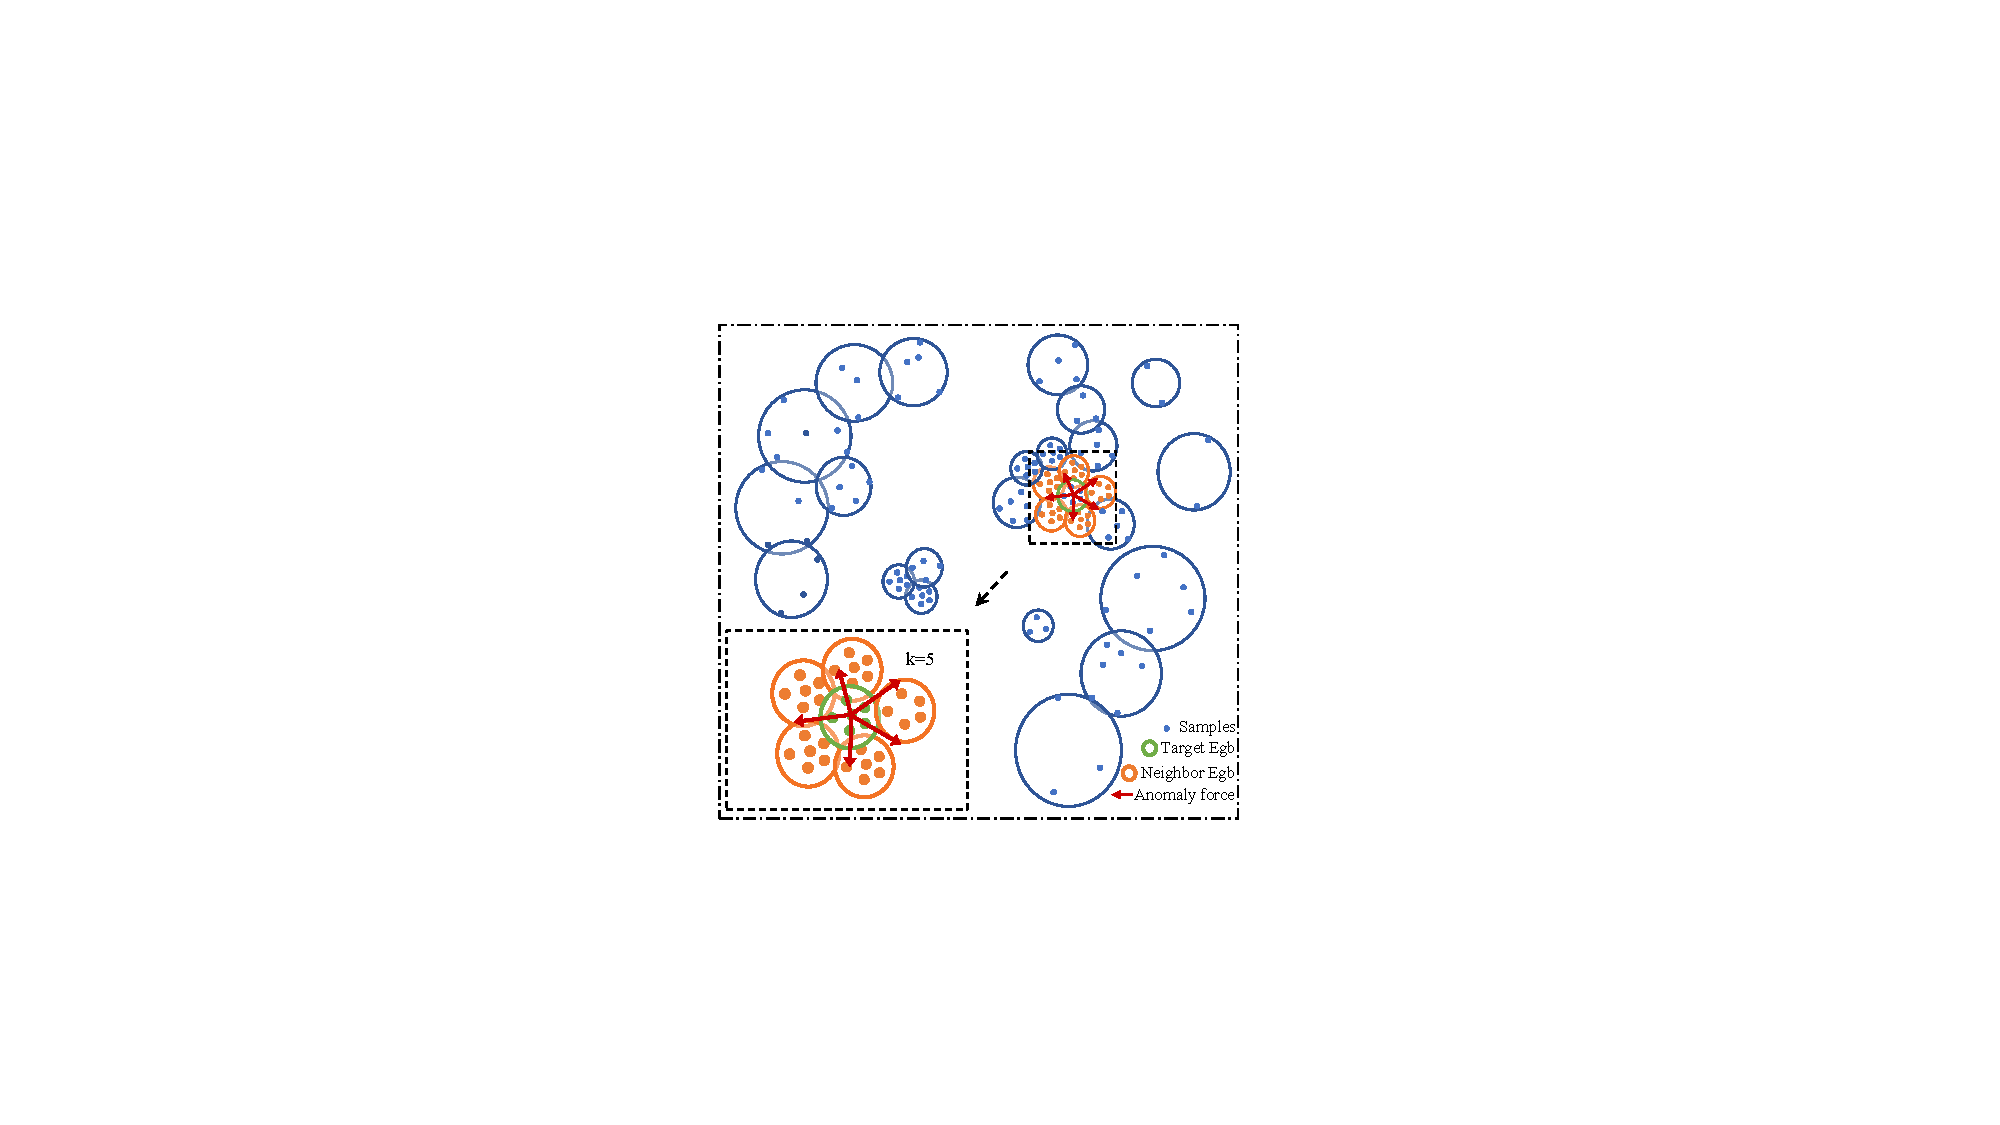
\includegraphics[scale=0.6]{denser_area.pdf}}
	\hspace{0.1in}
	\subfigure[Anomaly force in a sparse region]{
		\label{fig:Resultant Coulomb force}
		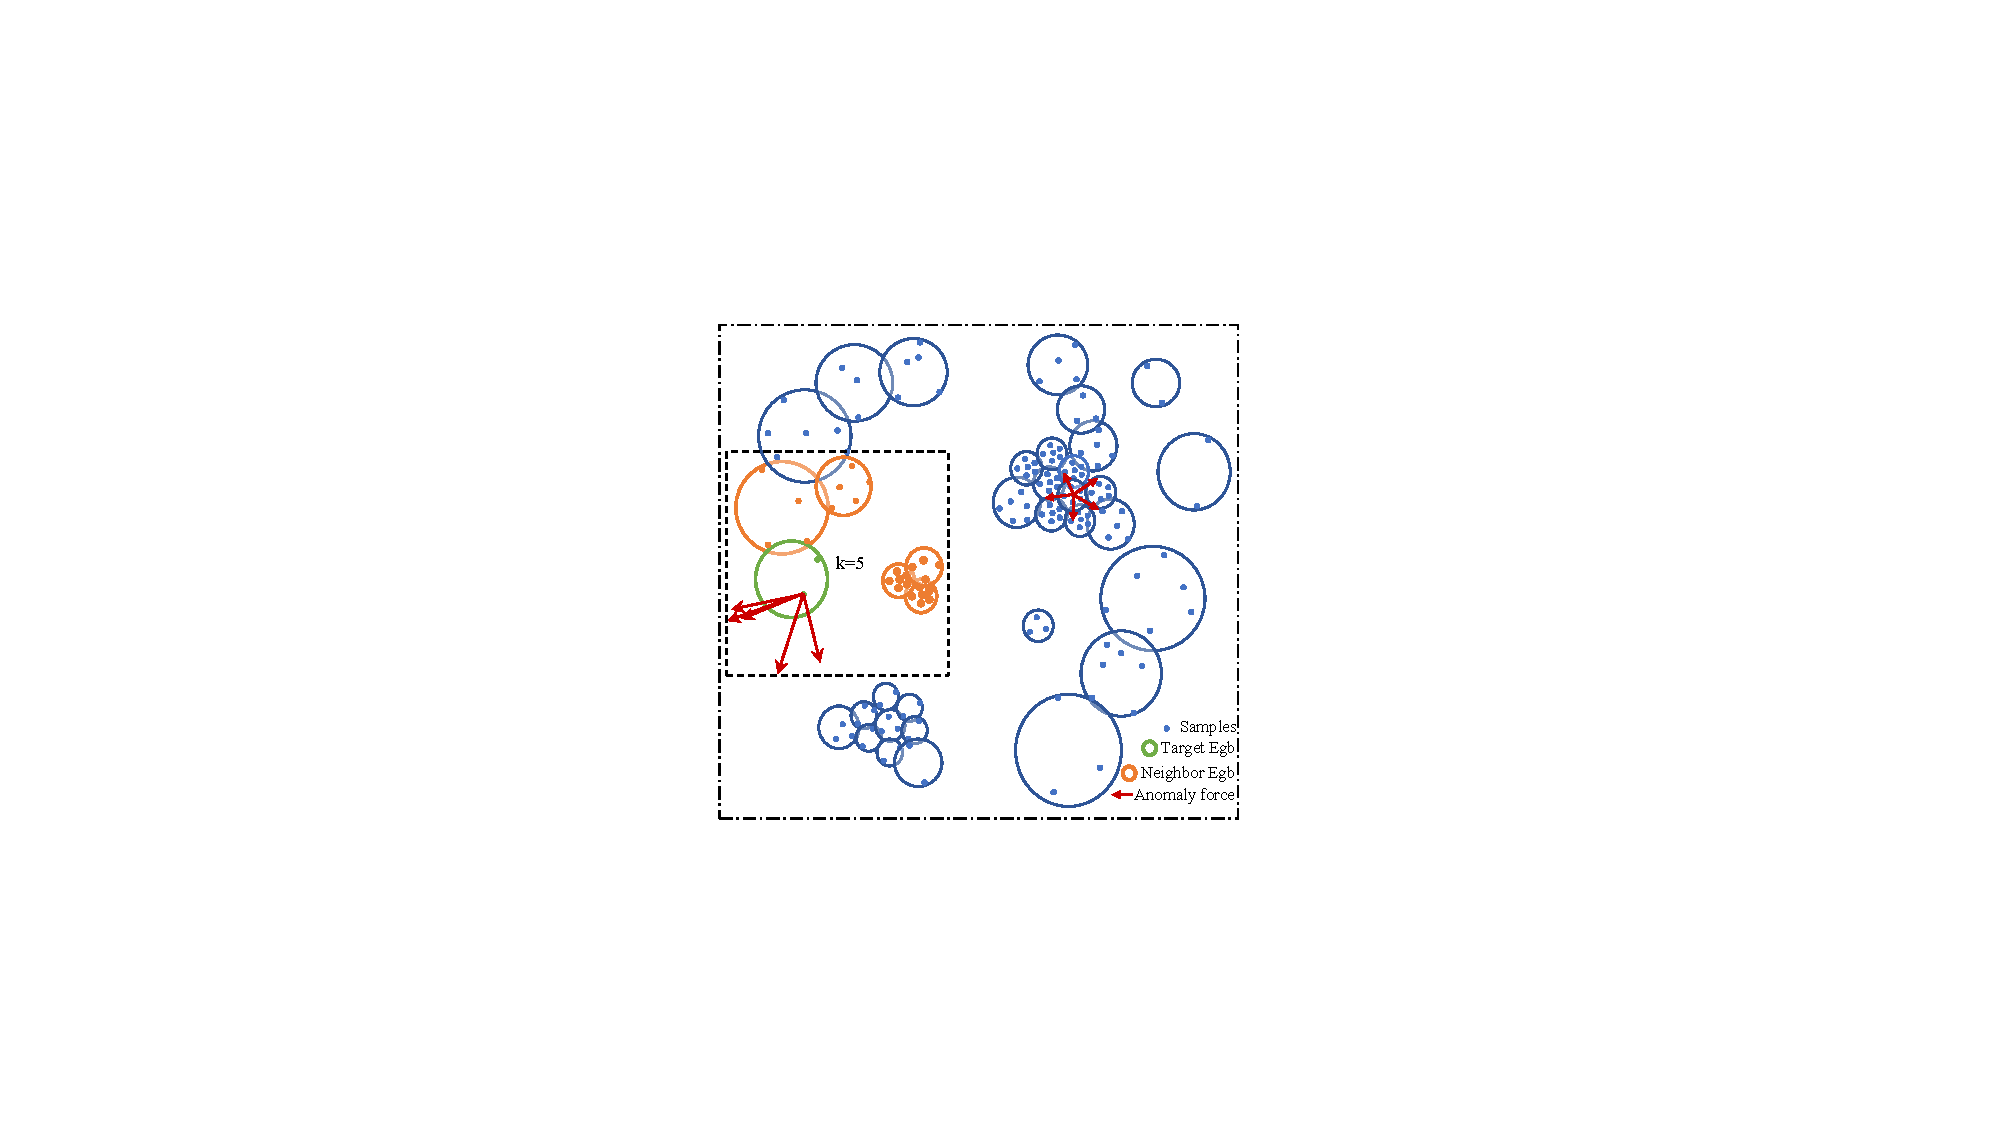
\includegraphics[scale=0.6]{sparser_area.pdf}}
	\caption{Illustration of the granular-ball anomaly force mechanism.}
	\label{fig:illustration for Coulomb force}
\end{figure*}

\subsection{Fusion strategy}

In this section, we propose the final anomaly score, which fuses global and local structural information.

\begin{definition}
    The final Anomaly Score ($AS$) for a sample $\boldsymbol{x} \in gb_i$ is defined as a linear combination of the normalized global and local scores:
\begin{equation}
    AS(\boldsymbol{x}) = \alpha \frac{LAS(\boldsymbol{x})-\min(LAS)}{\max(LAS)-\min(LAS)} + (1-\alpha) \frac{GAS(gb_i)-\min(GAS)}{\max(GAS)-\min(GAS)},
    \label{eq:anomaly score}
\end{equation}
where $\alpha \in [0,1]$ is a trade-off parameter. A higher $AS$ signifies a strong likelihood of abnormality, characterized by both intense local repulsion and global structural sparsity.
\end{definition}


The overall procedure of computing the $AS$ is summarized in Algorithm \ref{GBNAD-alg3}.

\begin{algorithm}[!htpb]
		\caption{Calculation of Anomaly Scores}
            \label{GBNAD-alg3}
		\LinesNumbered
		\KwIn{$EBS$, $kNN$ of $EBS$, $NaN$ of $EBS$, Dataset $\boldsymbol{X}$, $\alpha$, $k$;}
		\KwOut{Final Anomaly Scores;}
            \For{\textbf{each} $Egb \in EBS$}{
                Compute density $\rho$ via Eq. (\ref{eq:rho})\;
                Compute fuzzy density via Eq. (\ref{eq:fuzzy density})\;
                Compute global anomaly degree $GAS(Egb)$ via Eq. (\ref{eq:coarse-grained degree})\;
                \For{\textbf{each} $\boldsymbol{x}_i \in Egb$}{
                $GAS(\boldsymbol{x}_i) \leftarrow GAS(Egb)$\;
                }
            }
            \For{\textbf{each} $\boldsymbol{x}_i \in \boldsymbol{X}$}{
                $\boldsymbol{F} \leftarrow \boldsymbol{0}$\;
                Identify $Egb(\boldsymbol{x}_i)$ such that $\boldsymbol{x}_i \in Egb(\boldsymbol{x}_i)$\;
                $kNN(\boldsymbol{x}_i) \leftarrow kNN(Egb(\boldsymbol{x}_i))$\;
                \For{\textbf{each} $Egb_j \in kNN(\boldsymbol{x}_i)$}{
                    Calculate force $\boldsymbol{F}(\boldsymbol{x}_i, Egb_j)$ via Eq. (\ref{eq:Coulomb force between gb and xi})\;
                    $\boldsymbol{F} \leftarrow \boldsymbol{F} + \boldsymbol{F}(\boldsymbol{x}_i, Egb_j)$\;
                }
                Calculate $LAS(\boldsymbol{x}_i)$ via Eq. (\ref{eq:Coulomb resultant force of xi})\;
                Calculate final score $AS(\boldsymbol{x}_i)$ via Eq. (\ref{eq:anomaly score})\;
            }
            \Return {Anomaly Scores}.
\end{algorithm}

\begin{definition}
    Given an anomaly threshold $\varphi$, a sample $\boldsymbol{x}$ is classified as an anomaly if $AS(\boldsymbol{x}) > \varphi$.
\end{definition}

This definition translates the continuous anomaly scores into practical binary decisions. In practice, $\varphi$ acts as a sensitivity filter: a higher threshold reduces false alarms, while a lower threshold ensures fewer missed anomalies. Users can flexibly adjust $\varphi$ according to the estimated contamination rate or specific requirements of the application scenario.

\subsection{Time complexity analysis}

Assume the dataset $\boldsymbol{X}$ has a shape of $n \times d$. The construction of $EBS$ (containing $s$ balls, where $s \ll n$) using a KD-tree requires $O(n \log n)$ \cite{xie2023efficient}.
For the global score, identifying natural neighbors and computing fuzzy relations among $s$ granular-balls requires $O(s \log s)$ and $O(s^2)$, respectively. Thus, the global module complexity is $O(s^2)$.
For the local score, the computation of force has a time complexity of $O(nk)$.
Since $s \ll n$ and $k$ is a small constant, the overall time complexity is dominated by the granular-ball generation phase, i.e., $O(n \log n)$. This confirms the scalability of GBNAD for large-scale datasets.

\section{Experiments}
\label{Experiments}
% 在本节中，我们对13种算法进行了充分的比较研究，以显示GBNAD算法的优越性能。此外，我们还分析了属性噪声对算法的AUC的影响，参数的灵敏度以及模型中不同模块的贡献。在实验开始前，需要进行数据集准备、实验参数设置、评价指标建立等准备工作。
In this part, we conduct a comprehensive comparison between GBNAD and thirteen existing methods, highlighting the notable advantages and effectiveness of GBNAD. We further investigate the impact of attribute noise and conduct a sensitivity analysis of GBNAD. In addition, ablation experiments are performed to evaluate the individual contributions of each component within the GBNAD framework. Before conducting the experiments, we prepare the datasets, parameter settings, and establish the assessment criteria.
\subsection{Settings of experiments}
% 数据集介绍：种类、属性数量、数据集大小
% 对比的方法，方法的参数设置，对比的实验指标
In this work, we conducted extensive experiments and comparative analyses using 16 publicly available real-world datasets\footnote{https://github.com/BELLoney/Outlier-detection}. The detailed characteristics of these datasets are presented in Table \ref{The details of datasets.}. Each dataset contains a different quantity of samples (from $111$ to $9172$), attributes (from $4$ to $279$), and outliers (from $5$ to $258$), as well as the proportion of outliers in the dataset (from $0.44\%$ to $14.60\%$). To unify the data format, we normalize all attribute values to the [0,1] interval by min-max normalization. These datasets encompass a wide range of domains and attribute types, which allows us to thoroughly evaluate the performance of the GBNAD algorithm in various application scenarios.
% 在本项研究工作中，我们对20个公开可获取的真实数据集进行了详尽的数值实验和对比分析。表1中列出了这些数据集的详细特征。每个数据集包含不同数量的对象（数量介于107至9172之间）、属性（数量介于4至279之间）、异常值（数量介于5至2036之间），以及各自数据集中异常值所占的比例（比例介于0.44\%至14.60\%）。为了统一数据格式，我们通过最小-最大归一化处理将所有属性值标准化至[0,1]区间。这些数据集覆盖了多样化的领域和属性类型，从而使得我们能够在多种不同的应用场景下，全面评估GBNAD算法的性能表现。

We compared the GBNAD algorithm on the above 16 datasets with 13 other algorithms. Table \ref{The details of algorithms.} shows the detailed information about the algorithms used in the experiments, containing their names, key parameters, parameter settings, and computational complexity.

\begin{table}[!htb]
\centering
\caption{{The detailed information of datasets.}}
\label{The details of datasets.}
\resizebox{\linewidth}{!}{
\begin{tabular}{@{}clccccc@{}}
\toprule
{ No.} & \multicolumn{1}{c}{{ Names}}             & { Abbr.} & { Features} & { samples} & { Outliers} & { Outlier ratios} \\ \midrule
{ 1}   & { Yeast\_ERL\_5\_variant1}               & { Yeas}  & { 8}        & { 1141}    & { 5}        & { 0.44\%}         \\
{ 2}   & { Autos\_variant1}                       & { Autos} & { 25}       & { 205}     & { 25}       & { 12.20\%}        \\
{ 3}   & { Iris\_Irisvirginica\_11\_variant1}     & { Iris}  & { 4}        & { 111}     & { 11}       & { 9.91\%}         \\
{ 4}   & { Bands\_band\_16\_variant1}             & { Ban16} & { 39}       & { 328}     & { 16}       & { 4.88\%}         \\
{ 5}   & { Abalone\_variant1}                     & { Abal}  & { 8}        & { 4177}    & { 79}       & { 1.89\%}         \\
{ 6}   & { Cardiotocography\_2and3\_33\_variant1} & { Card}  & { 21}       & { 1688}    & { 33}       & { 1.95\%}         \\
{ 7}   & { Bands\_band\_34\_variant1}             & { Ban34} & { 39}       & { 346}     & { 34}       & { 9.83\%}         \\
{ 8}   & { Wbc\_malignant\_39\_variant1}          & { Wbc}   & { 9}        & { 483}     & { 39}       & { 8.07\%}         \\
{ 9}   & { Wdbc\_M\_39\_variant1}                 & { Wdbc}  & { 31}       & { 396}     & { 39}       & { 9.85\%}         \\
{ 10}  & { Bands\_band\_42\_variant1}             & { Ban42} & { 39}       & { 354}     & { 42}       & { 11.86\%}        \\
{ 11}  & { Arrhythmia\_variant1}                  & { Arrh}  & { 279}      & { 452}     & { 66}       & { 14.60\%}        \\
{ 12}  & { Satimage2}                             & { Sati}  & { 36}       & { 5803}    & { 71}       & { 1.22\%}         \\
{ 13}  & { Pendigits}                             & { Pend}  & { 16}       & { 6870}    & { 156}      & { 2.27\%}         \\
{ 14}  & { Thyroid\_disease\_variant1}            & { Thyr}  & { 28}       & { 9172}    & { 74}       & { 0.81\%}         \\
{ 15}  & { Musk}                                  & { Musk}  & { 166}      & { 3062}    & { 97}       & { 3.17\%}         \\
{ 16}  & { Pageblocks\_1\_258\_variant1}          & { Page}  & { 10}       & { 5171}    & { 258}      & { 4.99\%}         \\ \bottomrule
\end{tabular}%
}
\end{table}

\begin{table}[!htb]
\centering
\caption{{The detailed information of algorithms.}}
\label{The details of algorithms.}
\resizebox{\textwidth}{!}{
\begin{tabular}{@{}cllll@{}}
\toprule
{ No.} & { Names (Year)}                                         & { Time complexities} & { Parameters} & { Ranges of parameters}                           \\ \midrule
{ 1}   & { WDOD(2014) \cite{zhao2014simple}}    & { $O(mn)$}           & { $None$}     & { $None$}                                         \\
{ 2}   & { NOF(2016) \cite{ huang2016non}}      & { $O(n\log n)$}      & { $None$}     & { $None$}                                         \\
{ 3}   & { SRO(2017) \cite{you2017provable}}    & { $O(n^2t)$}         & { $\alpha$}   & { $[2,20]$}                                       \\
{ 4}   & { NC(2018) \cite{li2018outlier}}       & { $O(n^2)$}          & { $k$}        & { $[2,60]$}                                       \\
{ 5}   & { VarE(2020) \cite{li2018outlier}}     & { $O(n^2m)$}         & { $\lambda$}  & { $\{10^{-3},10^{-2},10^{-1},1,10^1,10^2,10^3\}$} \\
{ 6}   & { WNINOD(2021) \cite{wang2021outlier}} & { $O(n^2m+n^2t)$}    & { $\theta$}   & { $[1,10]$}                                       \\
{ 7}   & { MOD+(2021) \cite{yang2021mean}}      & { $O(n^2m)$}         & { $k,l$}      & { $[2,60];~l=3$}                                  \\
{ 8}   & { DCROD(2022) \cite{li2022robust}}     & { $O(nm\log n)$}     & { $k$}        & { $[2,60]$}                                       \\
{ 9}   & { ECOD(2022) \cite{li2022ecod}}                                           & { $O(mn)$}                  & { $None$}           & { $None$}                                              \\
{ 10}  & { ILGNI(2023) \cite{li2023incomplete}} & { $O(n^2+mn)$}       & { $a,b$}      & { $a=1;~b=100$}                                   \\
{ 11}  & { MFGAD(2023) \cite{yuan2023mfgad}}                                          & { $O(mn^2)$}                  & { $\sigma$}   & { $[0.1,2]$}                                      \\
{ 12}  & { NHOD(2023) \cite{zhu2022high}}       & { $O(n^2)$}          & { $k$}        & { $[2,60]$}                                       \\
{ 13}  & { MFIOD(2025) \cite{chen2024fusing}}                                                & { $O(n^2)$}                  & { $\lambda$}           & { $[0.05,1]$}                                               \\
{ 14}  & { GBNAD (Ours)}                                         & { $O(n\log n)$}      & { $k,\alpha$} & { $[2,60];~(0,1)$}                                \\ \bottomrule
\end{tabular}%
}
\end{table}


\subsection{Detection results analysis}
To evaluate the effectiveness of the models, the receiver operating characteristic (ROC) curve is adopted along with its area under the curve (AUC) \cite{yuan2023anomaly}.
The ROC curve reflects how the true positive rate (TPR) varies with the false positive rate (FPR) across various thresholds, offering a broad perspective on detection capability. 
However, the ROC curve may lack sufficient resolution when the performance of models is similar. Hence, we rely on AUC as a numerical indicator to enable more accurate and objective comparisons.
The AUC value is defined within the range of 0 to 1, and a value close to 1 is regarded as indicative of strong detection capability, reflecting the effectiveness of the model.
% 我们使用受试者工作特征曲线(ROC)和曲线下面积(AUC)来评估模型的性能。ROC曲线说明了不同决策阈值下的真阳性率(TPR)和假阳性率(FPR)之间的关系，提供了模型性能的全面视图。虽然ROC曲线是一个有用的可视化工具，但它在多个模型性能相近的情况下并不总是能够清楚地表明更好的算法。因此，我们也使用AUC作为定量指标来仔细比较算法性能。AUC的取值范围为$0\sim1$，接近1的值表示检测能力较好，即模型可以有效地识别数据中的异常值。

Fig. \ref{fig:roc} displays the ROC curves of various algorithms, each distinguished by a unique color and style. In general, the closer an ROC curve is to the top-left corner, the better the performance achieved by the algorithm. The ROC curve for the GBNAD algorithm is represented by pink diamond markers. According to Fig. \ref{fig:roc}, we have the following findings.

\begin{figure}[!htb]
\centering
% 左、下、右、上
\subfigure[Cardio]{

\includegraphics[width=0.24\textwidth,
trim=0.05cm 0.35cm 0.1cm 0.1cm,clip]
{cardiotocography_2and3_33_variant1_ROC.pdf}}
\hspace{-0.1in}
\subfigure[Iris]{
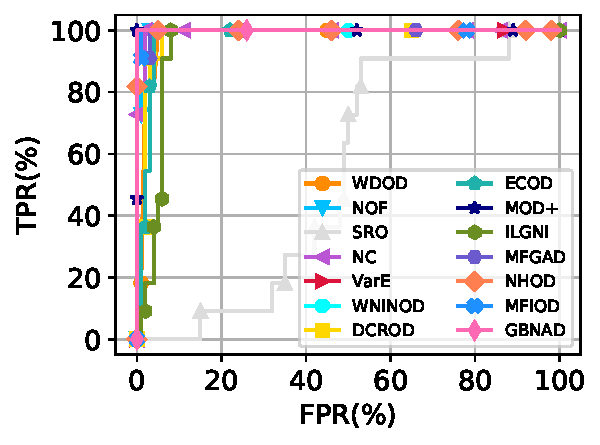
\includegraphics[width=0.24\textwidth,
trim=0.05cm 0.35cm 0.1cm 0.1cm,clip]
{iris_Irisvirginica_11_variant1_ROC.pdf}}
\hspace{-0.1in}
\subfigure[Musk]{
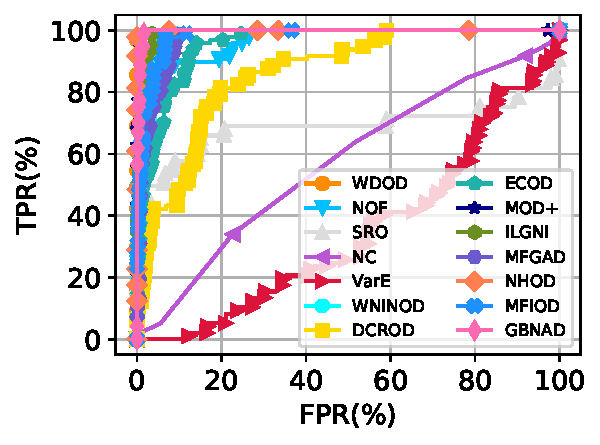
\includegraphics[width=0.24\textwidth,
trim=0.05cm 0.35cm 0.1cm 0.1cm,clip]
{musk_ROC.pdf}}
\hspace{-0.1in}
\subfigure[Page]{

\includegraphics[width=0.24\textwidth,
trim=0.05cm 0.35cm 0.1cm 0.1cm,clip]
{pageblocks_1_258_variant1_ROC.pdf}}
\\[-1ex]

\subfigure[Pend]{
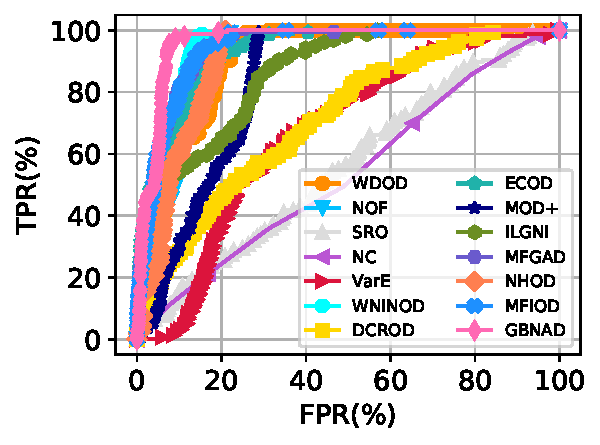
\includegraphics[width=0.24\textwidth,
trim=0.05cm 0.35cm 0.1cm 0.1cm,clip]
{pendigits_ROC.pdf}}
\hspace{-0.1in}
\subfigure[Sati]{
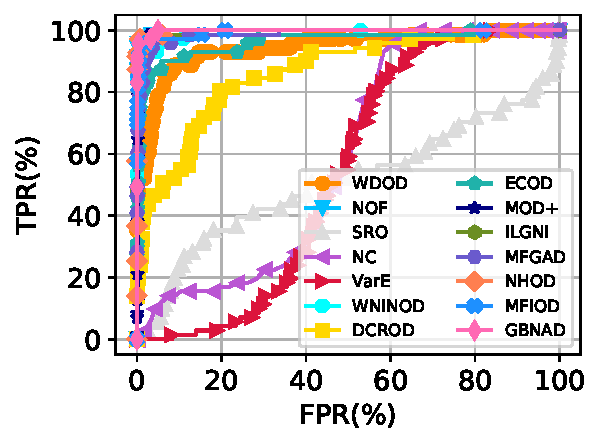
\includegraphics[width=0.24\textwidth,
trim=0.05cm 0.35cm 0.1cm 0.1cm,clip]
{satimage2_ROC.pdf}}
\hspace{-0.1in}
\subfigure[Wbc]{

\includegraphics[width=0.24\textwidth,
trim=0.05cm 0.35cm 0.1cm 0.1cm,clip]
{wbc_malignant_39_variant1_ROC.pdf}}
\hspace{-0.1in}
\subfigure[Wdbc]{
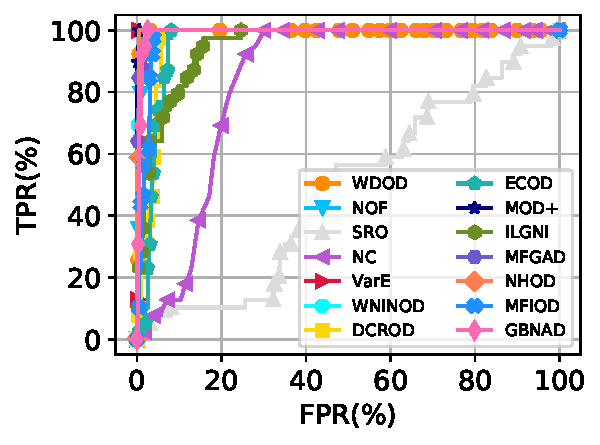
\includegraphics[width=0.24\textwidth,
trim=0.05cm 0.35cm 0.1cm 0.1cm,clip]
{wdbc_M_39_variant1_ROC.pdf}}
\\[-1ex]

\subfigure[Yeas]{
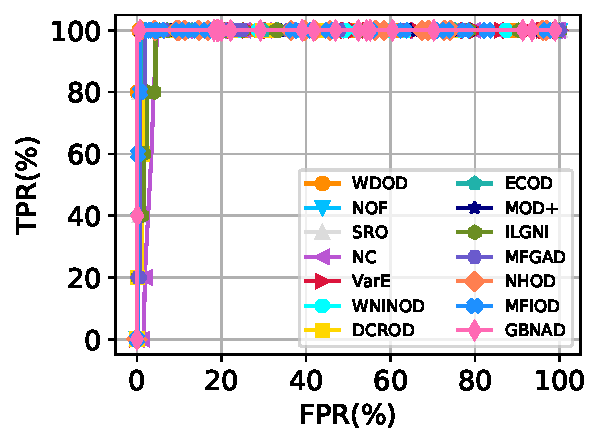
\includegraphics[width=0.24\textwidth,
trim=0.05cm 0.35cm 0.1cm 0.1cm,clip]
{yeast_ERL_5_variant1_ROC.pdf}}
\hspace{-0.1in}
\subfigure[Abal]{

\includegraphics[width=0.24\textwidth,
trim=0.05cm 0.35cm 0.1cm 0.1cm,clip]
{abalone_variant1_ROC.pdf}}
\hspace{-0.1in}
\subfigure[Arrh]{

\includegraphics[width=0.24\textwidth,
trim=0.05cm 0.35cm 0.1cm 0.1cm,clip]
{arrhythmia_variant1_ROC.pdf}}
\hspace{-0.1in}
\subfigure[Autos]{

\includegraphics[width=0.24\textwidth,
trim=0.05cm 0.35cm 0.1cm 0.1cm,clip]
{autos_variant1_ROC.pdf}}
\\[-1ex]

\subfigure[Ban16]{

\includegraphics[width=0.24\textwidth,
trim=0.05cm 0.35cm 0.1cm 0.1cm,clip]
{bands_band_16_variant1_ROC.pdf}}
\hspace{-0.1in}
\subfigure[Ban34]{

\includegraphics[width=0.24\textwidth,
trim=0.05cm 0.35cm 0.1cm 0.1cm,clip]
{bands_band_34_variant1_ROC.pdf}}
\hspace{-0.1in}
\subfigure[Ban42]{

\includegraphics[width=0.24\textwidth,
trim=0.05cm 0.35cm 0.1cm 0.1cm,clip]
{bands_band_42_variant1_ROC.pdf}}
\hspace{-0.1in}
\subfigure[Thyr]{

\includegraphics[width=0.24\textwidth,
trim=0.05cm 0.35cm 0.1cm 0.1cm,clip]
{thyroid_disease_variant1_ROC.pdf}}

\caption{ROC Curves for various datasets.}
\label{fig:roc}

\end{figure}

\begin{enumerate}[\indent(1)]
    \item {As observed, on datasets like Iris, Page, Pend and Sati, the ROC curves of GBNAD nearly align with the axes, indicating excellent performance.}
    \item {Besides, on datasets like Wdbc, Yeas, and Ban16, the ROC results of GBNAD are closest to the top-left corner, further demonstrating its strong performance.}
    \item {However, on datasets like Musk and Arrh, the curves of GBNAD coincide with those of several methods, which hinders a clear visual comparison of them.}
\end{enumerate}

Therefore, further quantitative evaluation using the AUC metric is necessary.
Table \ref{AUC results.} shows the results of the comparative experiments, listing the AUC values of 14 algorithms across 16 datasets. For each dataset, the highest AUC is \textbf{bold}. 
Based on the quantitative results presented in Table \ref{AUC results.}, we derive the following observations regarding the performance of GBNAD.
\begin{enumerate}[\indent(1)]
\item {GBNAD achieves the highest average AUC score of \textbf{0.900} across all 16 datasets. It secures the optimal performance on 9 out of 16 datasets. This consistent superiority indicates that GBNAD effectively adapts to diverse data distributions.}
\item Compared to existing physics-informed or neighborhood-based methods like NHOD and WNINOD, GBNAD demonstrates significant improvements. Specifically, on complex datasets such as {Card} and {Thyr}, GBNAD outperforms NHOD by margins of \textbf{5.8\%} and \textbf{17.5\%}, respectively. This validates our method overcomes the limitations of single-granularity PIML method, allowing the model to capture structural from global and local structure simultaneously.
\item The robustness of GBNAD is particularly evident on difficult datasets where traditional density-based methods struggle. For instance, on the {Thyr} dataset, classic algorithms like NOF (0.662) and WDOD (0.658) perform poorly. In contrast, GBNAD achieves a remarkable AUC of \textbf{0.750}, significantly outperforming the second-best method. This suggests that the fusion of global topological information and local physical interactions enables GBNAD to identify anomalies in complex structure.
\end{enumerate}

\begin{table*}[!htb]
\centering
\caption{{AUC results.}}
\label{AUC results.}
\resizebox{\textwidth}{!}{
\begin{tabular}{@{}ccccccccccccccc@{}}
\toprule
{Dataset} & {WDOD} & {NOF} & {SRO} & {NC} & {VarE} & {WNINOD} & {DCROD} & {ECOD} & {MOD+} & {ILGNI} & {MFGAD} & {NHOD} & {MFIOD} & {GBNAD} \\ \midrule
{Card} & {0.645} & {0.817} & {0.549} & {0.806} & {0.780} & {0.851} & {0.834} & {\textbf{0.871}} & {0.816} & {0.811} & {0.784} & {0.823} & {0.697} & {\textbf{0.871}} \\
{Iris} & {0.982} & {0.994} & {0.534} & {0.996} & {\textbf{1.000}} & {\textbf{1.000}} & {0.983} & {0.977} & {\textbf{1.000}} & {0.951} & {0.997} & {\textbf{1.000}} & {0.999} & {\textbf{1.000}} \\
{Musk} & {\textbf{1.000}} & {0.964} & {0.689} & {0.572} & {0.346} & {0.983} & {0.863} & {0.956} & {0.998} & {0.993} & {0.975} & {\textbf{1.000}} & {0.983} & {0.997} \\
{Page} & {0.837} & {0.963} & {0.870} & {0.803} & {0.727} & {0.956} & {0.953} & {0.938} & {0.963} & {0.914} & {0.655} & {0.977} & {0.922} & {\textbf{0.980}} \\
{Pend} & {0.097} & {0.909} & {0.562} & {0.537} & {0.665} & {0.939} & {0.712} & {0.927} & {0.832} & {0.862} & {0.941} & {0.907} & {0.944} & {\textbf{0.963}} \\
{Sati} & {0.058} & {0.999} & {0.512} & {0.590} & {0.537} & {0.988} & {0.865} & {0.965} & {0.996} & {0.994} & {0.989} & {\textbf{0.999}} & {0.995} & {{0.998}} \\
{Wbc} & {0.993} & {0.997} & {0.870} & {0.756} & {\textbf{0.997}} & {0.997} & {0.976} & {0.995} & {0.996} & {0.988} & {0.994} & {\textbf{0.997}} & {0.995} & {0.965} \\
{Wdbc} & {0.996} & {0.995} & {0.489} & {0.834} & {{0.997}} & {0.996} & {0.968} & {0.959} & {\textbf{1.000}} & {0.951} & {0.996} & {0.998} & {0.981} & {0.993} \\
{Yeas} & {0.999} & {\textbf{1.000}} & {0.995} & {0.970} & {\textbf{1.000}} & {0.998} & {0.990} & {0.995} & {\textbf{1.000}} & {0.981} & {0.992} & {\textbf{1.000}} & {0.996} & {0.999} \\
{Abal} & {0.690} & {{0.805}} & {0.783} & {0.729} & {{0.548}} & {0.641} & {0.780} & {0.653} & {{0.804}} & {0.604} & {0.565} & {{0.805}} & {0.642} & {\textbf{0.821}} \\
{Arrh} & {0.815} & {0.816} & {0.757} & {0.734} & {0.739} & {0.815} & {0.796} & {0.807} & {0.806} & {0.816} & {0.790} & {0.816} & {0.816} & {\textbf{0.836}} \\
{Autos} & {0.573} & {0.545} & {0.427} & {0.625} & {\textbf{0.819}} & {0.588} & {0.619} & {0.583} & {0.615} & {0.470} & {0.605} & {0.608} & {0.440} & {{0.740}} \\
{Ban16} & {0.712} & {0.825} & {0.392} & {0.793} & {{0.458}} & {0.859} & {0.864} & {\textbf{0.883}} & {0.817} & {0.780} & {0.816} & {0.811} & {0.649} & {0.879} \\
{Ban34} & {0.705} & {0.776} & {0.471} & {0.733} & {0.463} & {0.801} & {0.762} & {{0.782}} & {0.745} & {0.775} & {0.749} & {0.768} & {0.493} & {\textbf{0.808}} \\
{Ban42} & {0.706} & {0.787} & {0.408} & {0.732} & {0.496} & {0.785} & {0.756} & {0.750} & {0.757} & {0.743} & {0.748} & {0.755} & {0.449} & {\textbf{0.805}} \\
{Thyr} & {0.658} & {0.662} & {0.612} & {0.564} & {0.650} & {0.640} & {0.646} & {0.581} & {0.660} & {0.610} & {0.388} & {0.659} & {0.638} & {\textbf{0.750}} \\ \midrule
{Average} & {0.717} & {0.866} & {0.620} & {0.736} & {0.701} & {0.865} & {0.836} & {0.851} & {0.863} & {0.828} & {0.811} & {0.870} & {0.790} & {\textbf{0.900}} \\ 
{Average Rank} & {9.16} & {4.81} & {12.09} & {10.81} & {9.06} & {5.41} & {7.88} & {7.53} & {4.88} & {9.16} & {8.81} & {3.94} & {8.47} & {\textbf{3.00}} \\ \bottomrule
\end{tabular}%
}
\end{table*}

NHOD is one of the most representative methods among PIML-based methods as well as a single-granularity unsupervised method based on Coulomb's law, which has demonstrated excellent performance in anomaly detection, particularly on high-dimensional datasets. Therefore, to validate the improvement of our method, we conducted a comparison between GBNAD and NHOD on a two-dimensional synthetic dataset. The detection performance of both methods is illustrated in Fig. \ref{Visual results}.

\begin{figure}[!htb]
    \centering
    \subfigure[Visual result of NHOD]{
        \label{NHOD visual result}
        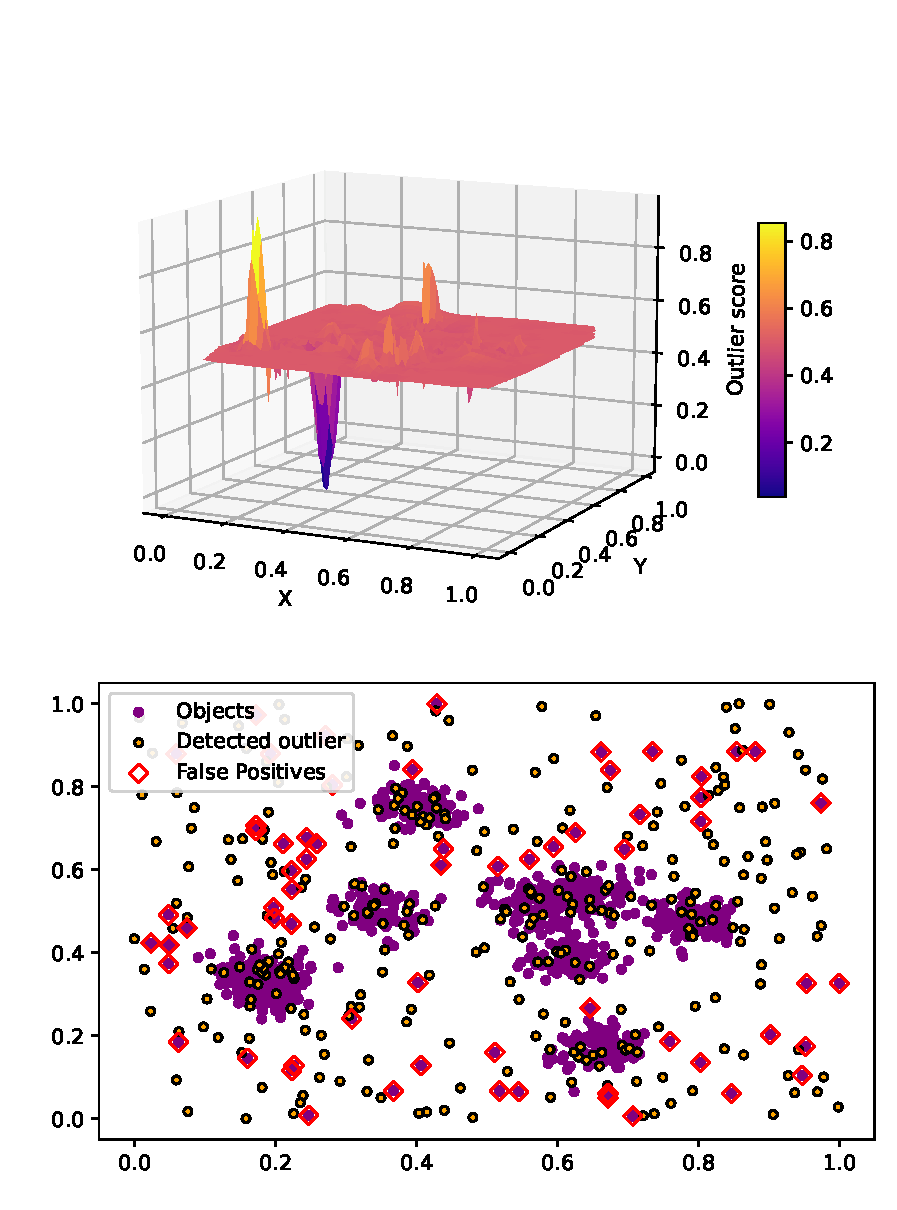
\includegraphics[width=0.45\textwidth]{NHOD_result.pdf}
    }
    % \hspace{-0.1in}
    \subfigure[Visual result of GBNAD]{
        \label{GBNAD visual result}
        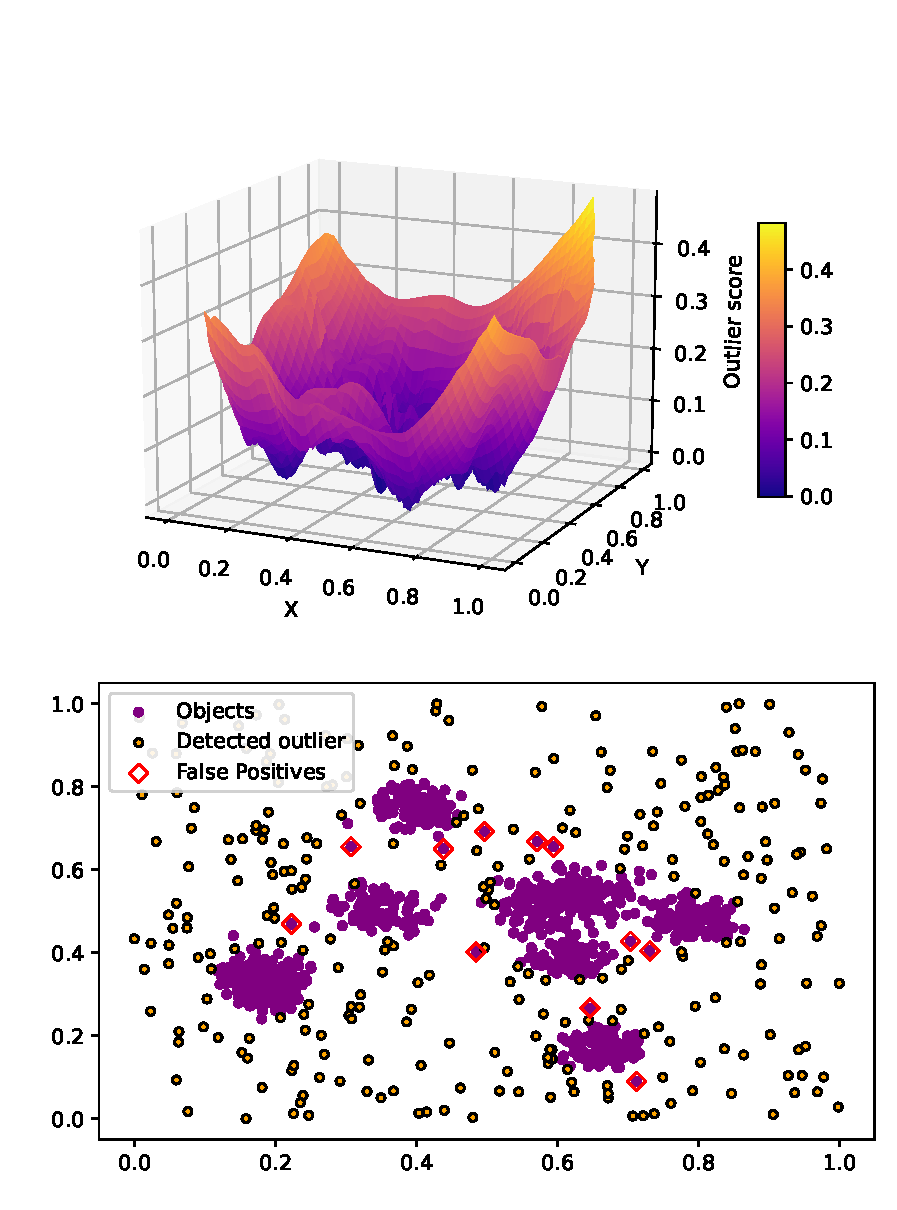
\includegraphics[width=0.45\textwidth]{GBNAD_result.pdf}
    }
\caption{Visual results.}
\label{Visual results}
\end{figure}

{The visualization consists of two parts. The top row presents the 3D surface plots of the anomaly score distribution, where the Z-axis represents the magnitude of the outlier score across the 2D spatial coordinates. The bottom row displays the detection results, where purple dots represent the samples, yellow dots represent the detected outliers. Additionally, the red diamonds indicate false positives, i.e., normal samples incorrectly classified as anomalies.}
Based on Fig. \ref{Visual results}, we derive the following findings.
\begin{enumerate}[\indent(1)]
    \item As shown in the 3D plots, the outlier score surface of NHOD is rugged with sharp, discontinuous peaks, indicating high sensitivity to local noise. In contrast, GBNAD exhibits a much smoother and continuous score landscape. 
    % The valleys align perfectly with normal clusters, while the scores rise gradually in sparse regions, demonstrating the superior robustness of GBNAD.
    
    \item In the 2D scatter plots, NHOD misclassifies a significantly higher number of samples as normal than GBNAD.
    
    \item The peak distribution of outliers in GBNAD closely aligns with the global clustering pattern of the data. This suggests that by shifting from point-wise interaction to granular-ball interaction, GBNAD captures the comprehensive data distribution more effectively than the fine-grained NHOD.
\end{enumerate}

To sum up, the results of extensive experiments validate that GBNAD is more effective in anomaly detection compared to the other methods, particularly surpassing single-perspective PIML method NHOD.
% 此外图\ref{Visual results}显示了NHOD算法和GBNAD算法的检测结果对比。从图中，我们可以得出以下结论：

% 1、AUC曲线图
% 2、根据结果看是否采用箱线图
% 3、算法运行时间对比（注意和baseline的比较）
% 4、抗噪性实验
% 5、算法参数分析
%   5.1 两个分数的融合参数alpha
%   5.2 邻居数量k
%   此外，还有距离的m次方



\subsection{Runtime analysis}
{In an assessment of our approach's computational efficiency, we recorded the execution times for GBNAD and the comparative algorithms.} The execution times across 16 datasets are reported in Table \ref{Runtime results (in seconds).}. GBNAD optimizes computational resources by using granular-balls in the anomaly force calculation. High-quality granular-balls enable GBNAD to bypass exhaustive pairwise distance calculations while maintaining detection accuracy, leading to outstanding runtime efficiency. As shown in Table \ref{Runtime results (in seconds).}, GBNAD achieves an average runtime of 0.809 seconds, ranking mid-range among all algorithms. However, the gap between GBNAD and the better ones is minimal, highlighting the efficiency of GBNAD.

\begin{table}[!htb]
\centering
\caption{Execution times (in seconds).}
\label{Runtime results (in seconds).}
\resizebox{\textwidth}{!}{
\begin{tabular}{@{}ccccccccccccccc@{}}
\toprule
{ Dataset} & { WDOD}                      & { NOF}                         & { SRO}                         & { NC}                        & { VarE}                       & { WNINOD}                      & { DCROD}                     & { ECOD}                               & { MOD+}                      & { ILGNI}                        & { MFGAD}                     & { NHOD}                      & { MFIOD}                     & { GBNAD (Ours)} \\ \midrule
{ Card}    & { 0.192}                     & { 36.841}                      & { 0.585}                       & { 0.639}                     & { 2.563}                      & { 10.257}                      & { 0.291}                     & { \textbf{0.004}}                     & { 1.436}                     & { 34.643}                       & { 0.784}                     & { 0.236}                     & { 0.979}                     & { 0.158}        \\
{ Iris}    & { 0.001}                     & { 0.147}                       & { 0.017}                       & { 0.005}                     & { 0.005}                      & { 0.002}                       & { 0.013}                     & { \textbf{0.001}}                     & { 0.064}                     & { 0.005}                        & { 0.997}                     & { 0.002}                     & { 0.745}                     & { 0.014}        \\
{ Musk}    & { 2.785}                     & { 852.359}                     & { 6.178}                       & { 5.580}                     & { 42.737}                     & { 552.755}                     & { 2.689}                     & { \textbf{0.092}}                     & { 6.304}                     & { 21308.749}                    & { 0.975}                     & { 4.801}                     & { 0.945}                     & { 1.703}        \\
{ Page}    & { 0.652}                     & { 337.488}                     & { 119.867}                     & { 1.419}                     & { 143.794}                    & { 195.719}                     & { 0.754}                     & { \textbf{0.009}}                     & { 3.611}                     & { 595.864}                      & { 0.655}                     & { 1.275}                     & { 0.981}                     & { 1.135}        \\
{ Pend}    & { 1.200}                     & { 1892.756}                    & { 21.952}                      & { 1.568}                     & { 232.747}                    & { 772.717}                     & { 2.838}                     & { \textbf{0.021}}                     & { 9.039}                     & { 2373.196}                     & { 0.941}                     & { 2.567}                     & { 0.752}                     & { 2.356}        \\
{ Sati}    & { 1.914}                     & { 2038.825}                    & { 30.220}                      & { 3.909}                     & { 138.815}                    & { 1188.166}                    & { 1.178}                     & { \textbf{0.029}}                     & { 8.831}                     & { 3879.356}                     & { 0.989}                     & { 3.695}                     & { 0.858}                     & { 1.378}        \\
{ Wbc}     & { 0.010}                     & { 11.054}                      & { 0.191}                       & { 0.041}                     & { 0.118}                      & { 0.089}                       & { 0.172}                     & { \textbf{0.001}}                     & { 0.315}                     & { 0.290}                        & { 0.994}                     & { 0.010}                     & { 0.893}                     & { 0.040}        \\
{ Wdbc}    & { 0.028}                     & { 2.986}                       & { 0.061}                       & { 0.064}                     & { 0.084}                      & { 0.133}                       & { 0.062}                     & { \textbf{0.002}}                     & { 0.213}                     & { 2.077}                        & { 0.996}                     & { 0.028}                     & { 0.912}                     & { 0.030}        \\
{ Yeas}    & { 0.022}                     & { 30.324}                      & { 1.852}                       & { 0.081}                     & { 0.765}                      & { 1.642}                       & { 0.141}                     & { \textbf{0.001}}                     & { 0.732}                     & { 6.325}                        & { 0.992}                     & { 0.053}                     & { 0.919}                     & { 0.091}        \\
{ Abal}    & { 0.355}                     & { 455.392}                     & { 1143.250}                    & { 0.346}                     & { 76.162}                     & { 108.677}                     & { 0.548}                     & { \textbf{0.005}}                     & { 2.992}                     & { 262.832}                      & { 0.565}                     & { 0.628}                     & { 0.832}                     & { 0.558}        \\
{ Arrh}    & { 0.440}                     & { 31.814}                      & { 1.824}                       & { 0.186}                     & { 0.319}                      & { 1.918}                       & { 0.239}                     & { \textbf{0.017}}                     & { 0.512}                     & { 1576.085}                     & { 0.790}                     & { 0.208}                     & { 0.903}                     & { 0.119}        \\
{ Autos}   & { 0.010}                     & { 0.944}                       & { 0.104}                       & { 0.006}                     & { 0.041}                      & { 0.021}                       & { 0.029}                     & { \textbf{0.001}}                     & { 0.094}                     & { 0.346}                        & { 0.605}                     & { 0.012}                     & { 0.392}                     & { 0.036}        \\
{ Ban16}   & { 0.023}                     & { 1.852}                       & { 1.503}                       & { 0.014}                     & { 0.142}                      & { 0.091}                       & { 0.024}                     & { \textbf{0.002}}                     & { 0.149}                     & { 2.807}                        & { 0.816}                     & { 0.019}                     & { 0.055}                     & { 0.022}        \\
{ Ban34}   & { 0.021}                     & { 2.011}                       & { 0.898}                       & { 0.018}                     & { 0.256}                      & { 0.103}                       & { 0.046}                     & { \textbf{0.002}}                     & { 0.188}                     & { 3.214}                        & { 0.749}                     & { 0.028}                     & { 0.058}                     & { 0.024}        \\
{ Ban42}   & { 0.018}                     & { 2.120}                       & { 0.932}                       & { 0.055}                     & { 0.205}                      & { 0.198}                       & { 0.044}                     & { \textbf{0.002}}                     & { 0.178}                     & { 3.914}                        & { 0.748}                     & { 0.030}                     & { 0.060}                     & { 0.020}        \\
{ Thyr}    & { 4.867}                     & { 6720.517}                    & { 10053.415}                   & { 3.080}                     & { 497.669}                    & { 4059.247}                    & { 3.603}                     & { \textbf{0.037}}                     & { 16.270}                    & { 10332.106}                    & { 0.388}                     & { 7.138}                     & { 0.959}                     & { 4.472}        \\ \midrule
{ Average} & {{ 0.784}} & {{ 776.089}} & {{ 711.428}} & {{ 1.063}} & {{ 71.026}} & {{ 430.734}} & {{ 0.792}} & {{ \textbf{0.014}}} & {{ 3.183}} & {{ 2523.863}} & {{ 0.811}} & {{ 1.296}} & {{ 0.703}} & { 0.809}        \\ \bottomrule
\end{tabular}%
}
\end{table}

{\subsection{Statical analysis}}

{
The Friedman test was first employed \cite{chen2025label} to validate the statistical significance of the performance differences between GBNAD and the comparative algorithms across 16 datasets. Based on the experimental setup, the degrees of freedom for the $F$-statistic are $13$ and $195$. At a significance level of $\alpha=0.1$, the calculated Friedman statistic yielded $\tau_F = 10.6376$, which is significantly larger than the critical value of $1.5585$. This result indicates that statistically significant differences exist among all compared algorithms, leading to the rejection of the null hypothesis.}

{
To further elucidate the specific differences between the algorithms, the Nemenyi post-hoc test was conducted, with the visualization results presented in Fig. \ref{fig:Nemenyi test figure on AUC}. The red scale at the top of the figure indicates a Critical Difference (CD) value of $4.6145$. As observed in Fig. \ref{fig:Nemenyi test figure on AUC}, GBNAD achieved the optimal average rank, demonstrating superior performance across the datasets. According to the Nemenyi test criteria, GBNAD significantly outperforms DCROD, SRO, NC, WDOD, ILGNI, VarE, MFGAD, and MFIOD, as the difference in their average ranks exceeds the CD value. However, despite its top ranking, GBNAD shares the same significance level with comparable methods such as MOD+ and NOF.}

\begin{figure}[!htb]
    \centering
    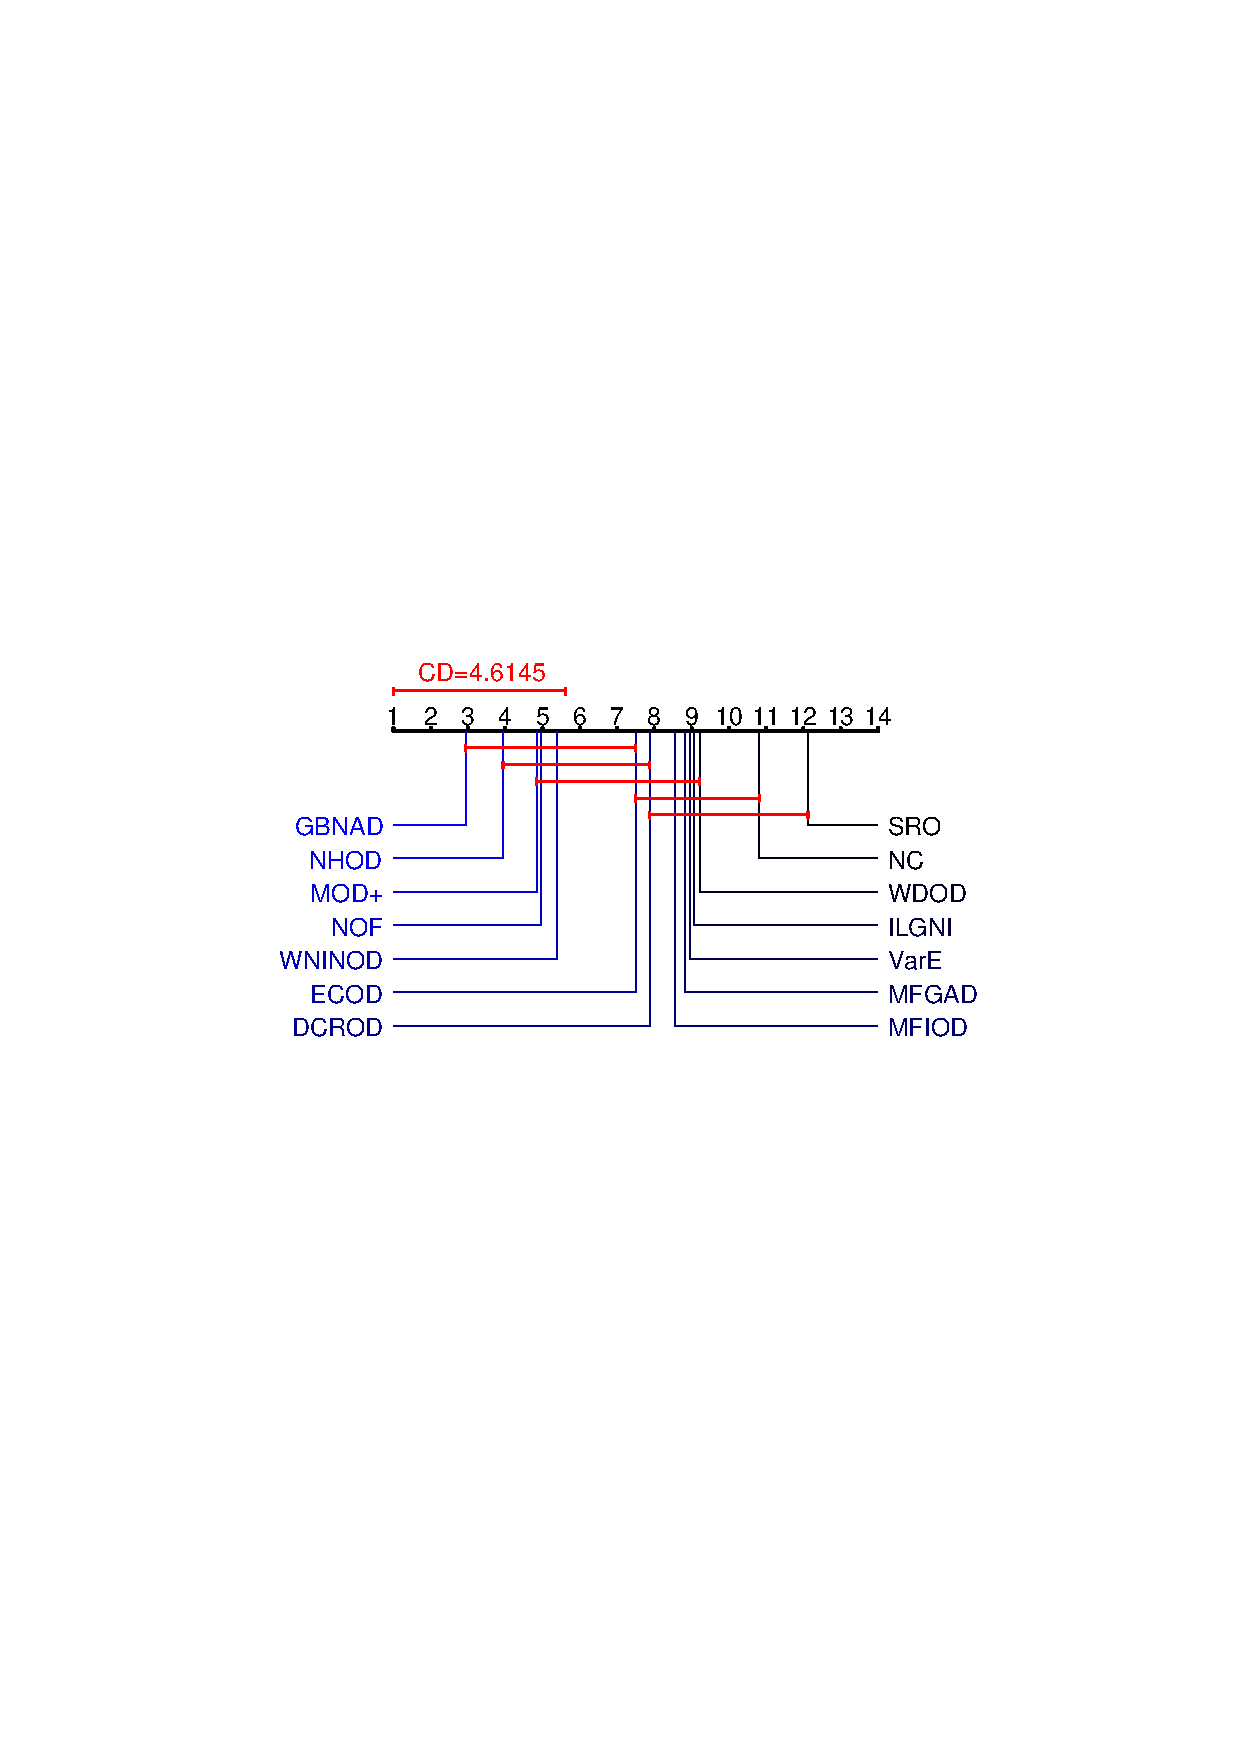
\includegraphics[width=0.5\linewidth]{outlier_results_GBNAD.pdf}
    \caption{{Nemenyi test figure on AUC.}}
    \label{fig:Nemenyi test figure on AUC}
\end{figure}

\subsection{Robustness analysis against attribute noise}
Following the methodology in \cite{yuan2023anomaly}, we evaluate the robustness of the algorithm to attribute noise.
To simulate real-world data corruption, we introduce random attribute noise by altering the values of $\lceil{t\%}\cdot{n}\rceil$ samples within a randomly selected attribute, where $t\%$ denotes the noise level. Specifically, the original values are replaced with uniform random noise derived from the attribute's valid range $[\min, \max]$. 
Fig. \ref{fig:noise} illustrates the impact of varying noise intensities on the detection performance of GBNAD.
As observed, although the AUC exhibits slight fluctuations as the noise level increases, the overall performance remains stable. This stability is particularly evident in datasets such as {Sati}, {Yeas}, and {Wdbc}. These results demonstrate the robustness of the proposed GBNAD algorithm, attributed to the coarse-grained nature of granular-balls which effectively filters out noise interference.

\begin{figure}[!htb]
    \centering
    \subfigure[datasets 1-8]{
        \label{dataset 1-10_noise}
        % \vspace{-2cm}
        % 左、下、右、上
        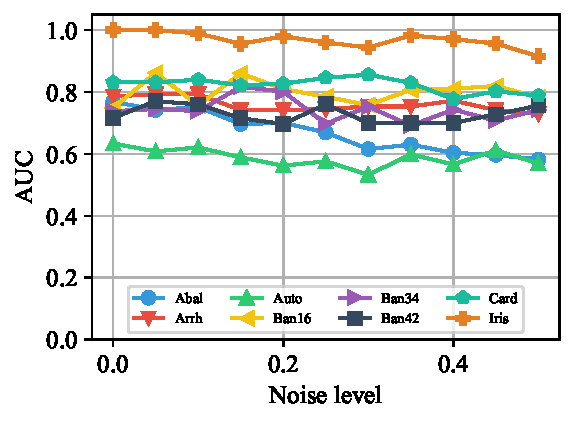
\includegraphics[width=0.4\textwidth,
trim=0.05cm 0.3cm 0.1cm 0.25cm,clip]{anti_noise_auc_1.pdf}
    }
    \hspace{-0.1in}
    \subfigure[datasets 9-16]{
        \label{dataset 11-20}
        % \vspace{-2cm}
        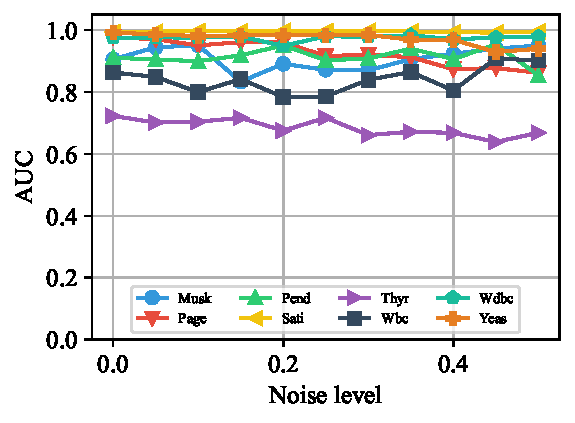
\includegraphics[width=0.4\textwidth,
trim=0.05cm 0.3cm 0.1cm 0.25cm,clip]{anti_noise_auc_2.pdf}
    }
    \caption{{Impact of varying attribute noise levels on AUC performance.}}
    \label{fig:noise}
\end{figure}

\subsection{Algorithm sensitivity analysis}
There are two tunable parameters included in GBNAD. Parameter $k$ defines the size of the neighborhood used during computation, while $\alpha$ adjusts the fuse strategy of the final anomaly score. Figs. \ref{fig:Variation curve of AUC with k.} and \ref{fig:Variation curve of AUC with alpha.} illustrate how the AUC value of the algorithm varies with changes in $k$ and $\alpha$.
As shown in Figs. \ref{dataset 1-10_parameter_k} and \ref{dataset 11-20_parameter_k}, the AUC value increases as the increase of $k$ across different datasets. While performance varies slightly among datasets, the overall trend remains consistent. In most cases, AUC increases and stabilizes after $k=20$, indicating that the increase of neighborhood included improves the algorithm performance. As $k$ continues to increase, the AUC value fluctuates slightly. Similarly, Figs. \ref{dataset 1-10_parameter_alpha} and \ref{dataset 11-20_parameter_alpha} show that AUC values also increase with $\alpha$, suggesting a positive effect on performance. However, compared to the effect of $k$, the fluctuations caused by $\alpha$ are smaller, indicating that the algorithm is less sensitive to changes of $\alpha$.

\begin{figure}[!htb]
    \centering
    \subfigure[$k$ on datasets 1-8]{
        \label{dataset 1-10_parameter_k}
        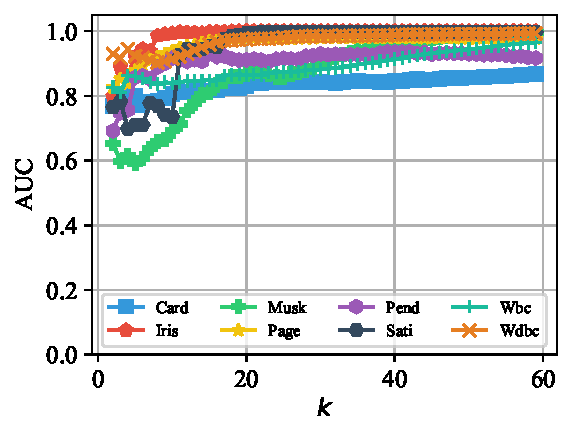
\includegraphics[width=0.4\textwidth,
trim=0.05cm 0.35cm 0.1cm 0.2cm,clip]{k_auc_1.pdf}
    }
    % \hspace{-0.1in}
    \subfigure[$k$ on datasets 9-16]{
        \label{dataset 11-20_parameter_k}
        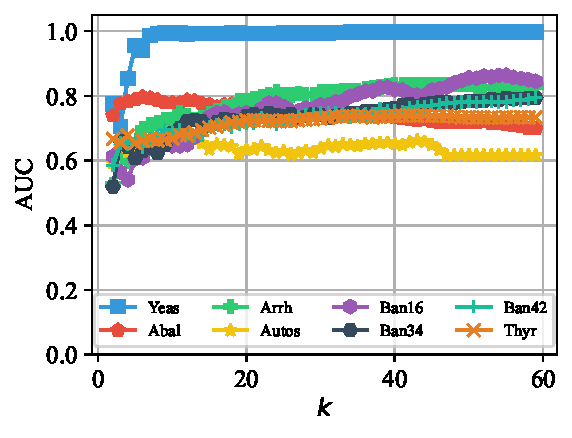
\includegraphics[width=0.4\textwidth,
trim=0.05cm 0.35cm 0.1cm 0.2cm,clip]{k_auc_2.pdf}
    }
    \caption{{Variation curves of AUC with $k$.}}
    \label{fig:Variation curve of AUC with k.}
\end{figure}

\begin{figure}[!htb]
    \centering
    \subfigure[$\alpha$ on datasets 1-8]{
        \label{dataset 1-10_parameter_alpha}
        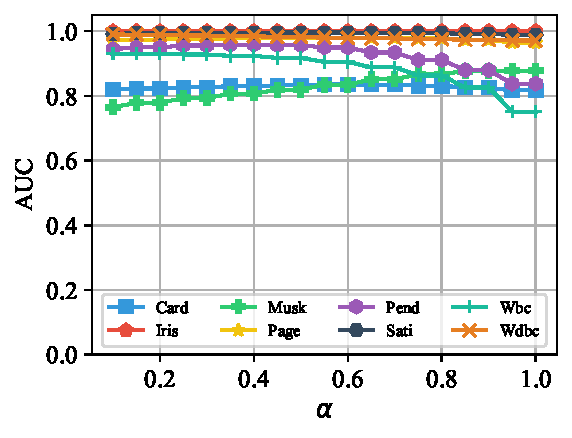
\includegraphics[width=0.4\textwidth,
trim=0.05cm 0.35cm 0.1cm 0.2cm,clip]{alpha_auc_1.pdf}
    }
    \subfigure[$\alpha$ on datasets 9-16]{
        \label{dataset 11-20_parameter_alpha}
        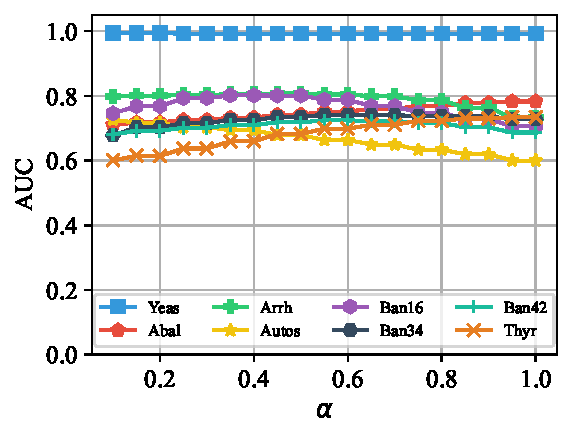
\includegraphics[width=0.4\textwidth,
trim=0.05cm 0.35cm 0.1cm 0.2cm,clip]{alpha_auc_2.pdf}
    }
    \caption{{Variation curves of AUC with $\alpha$.}}
    \label{fig:Variation curve of AUC with alpha.}
\end{figure}

\subsection{Ablation analysis}
The framework of GBNAD consists of two distinct modules: the global metric module (Module A) and the local metric module (Module B). Ablation experiments were conducted across 16 datasets to evaluate the individual contributions and interactions of the components. Fig. \ref{fig: Ablation experiments for various datasets} and Table \ref{Ablation_experiments_results} present the performance of the complete GBNAD algorithm (Module A+B) compared to its sub-modules. 

\begin{table}[!hb]
\centering
\caption{Quantitative comparison of runtime and AUC performance.}
\label{Ablation_experiments_results}
\resizebox{\linewidth}{!}{
\begin{tabular}{@{}c|ccc|ccc@{}}
\hline
{ }                           & \multicolumn{3}{c}{{ Runtime}}                                                          & \multicolumn{3}{c}{{ AUC}}                                                            \\ \cline{2-7} 
\multirow{-2}{*}{{ Datasets}} & { Module A+B} & { Module A}       & { Module B} & { Module A+B}     & { Module A} & { Module B} \\ \hline
{ Card}                       & { 0.179}      & { \textbf{0.075}} & { 0.148}    & { \textbf{0.873}} & { 0.803}    & { 0.859}    \\
{ Iris}                       & { 0.005}      & { \textbf{0.004}} & { 0.004}    & { \textbf{1.000}} & { 0.913}    & { 1.000}    \\
{ Musk}                       & { 1.870}      & { \textbf{0.222}} & { 1.663}    & { \textbf{0.997}} & { 0.749}    & { 0.996}    \\
{ Page}                       & { 1.136}      & { \textbf{0.039}} & { 1.035}    & { \textbf{0.980}} & { 0.957}    & { 0.952}    \\
{ Pend}                       & { 2.862}      & { \textbf{0.088}} & { 2.774}    & { \textbf{0.963}} & { 0.936}    & { 0.893}    \\
{ Sati}                       & { 1.500}      & { \textbf{0.043}} & { 1.368}    & { \textbf{0.999}} & { 0.976}    & { 0.995}    \\
{ Wbc}                        & { 0.046}      & { \textbf{0.021}} & { 0.039}    & { \textbf{0.964}} & { 0.888}    & { 0.961}    \\
{ Wdbc}                       & { 0.032}      & { \textbf{0.009}} & { 0.028}    & { \textbf{0.992}} & { 0.928}    & { 0.989}    \\
{ Yeas}                       & { 0.110}      & { \textbf{0.050}} & { 0.087}    & { \textbf{0.998}} & { 0.952}    & { 0.997}    \\
{ Abal}                       & { 0.844}      & { \textbf{0.145}} & { 0.668}    & { \textbf{0.821}} & { 0.702}    & { 0.820}    \\
{ Arrh}                       & { 0.122}      & { \textbf{0.012}} & { 0.109}    & { \textbf{0.828}} & { 0.781}    & { 0.806}    \\
{ Autos}                      & { 0.036}      & { \textbf{0.009}} & { 0.021}    & { \textbf{0.740}} & { 0.724}    & { 0.648}    \\
{ Ban16}                      & { 0.021}      & { \textbf{0.012}} & { 0.017}    & { \textbf{0.875}} & { 0.706}    & { 0.850}    \\
{ Ban34}                      & { 0.033}      & { \textbf{0.031}} & { 0.018}    & { \textbf{0.809}} & { 0.641}    & { 0.768}    \\
{ Ban42}                      & { 0.021}      & { \textbf{0.008}} & { 0.018}    & { \textbf{0.806}} & { 0.665}    & { 0.761}    \\
{ Thyr}                       & { 4.911}      & { \textbf{0.113}} & { 4.469}    & { \textbf{0.750}} & { 0.619}    & { 0.730}    \\ \hline
{ Average}                    & { 0.858}      & { \textbf{0.055}} & { 0.779}    & { \textbf{0.900}} & { 0.809}    & { 0.877}    \\ \hline
\end{tabular}%
}
\end{table}

\begin{figure}[!htb]
    \centering
    \subfigure[results on datasets 1-8]{
        \label{dataset 1-8_ablation}
        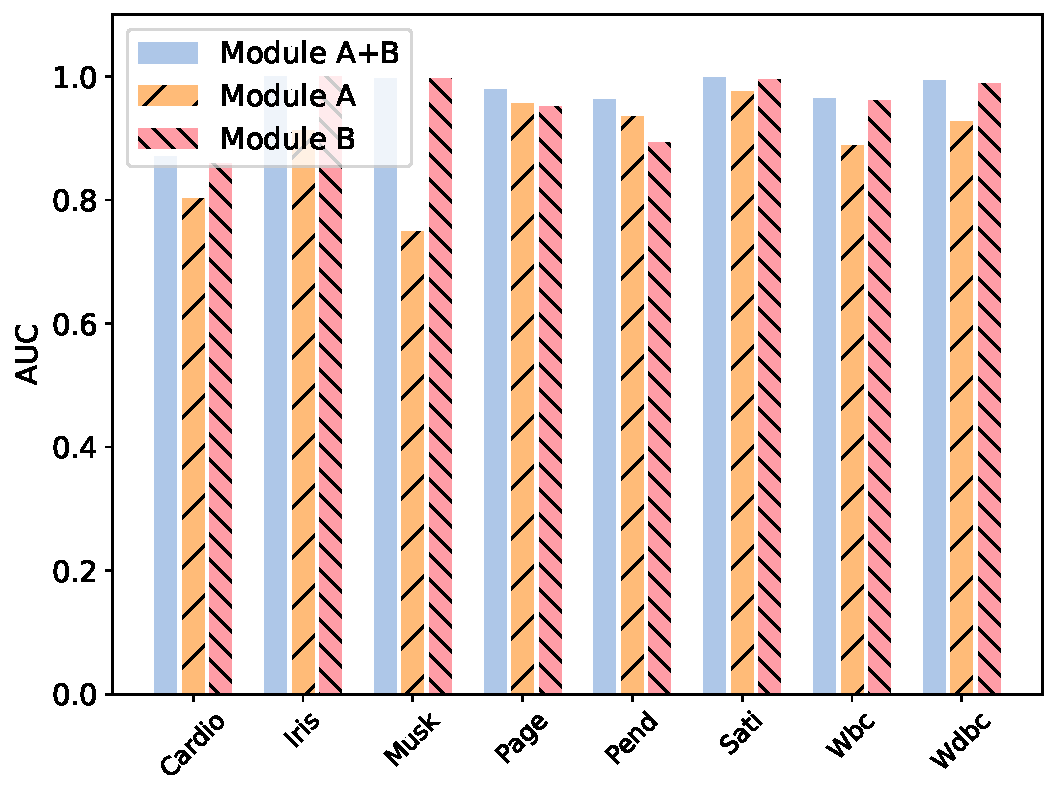
\includegraphics[width=0.45\textwidth,
trim=0.05cm 0.35cm 0.1cm 0.2cm,clip]{all_datasets_auc_values_0_8.pdf}
    }
    % \hspace{-0.2in}
    \subfigure[results on datasets 9-16]{
        \label{dataset 9-16_ablation}
        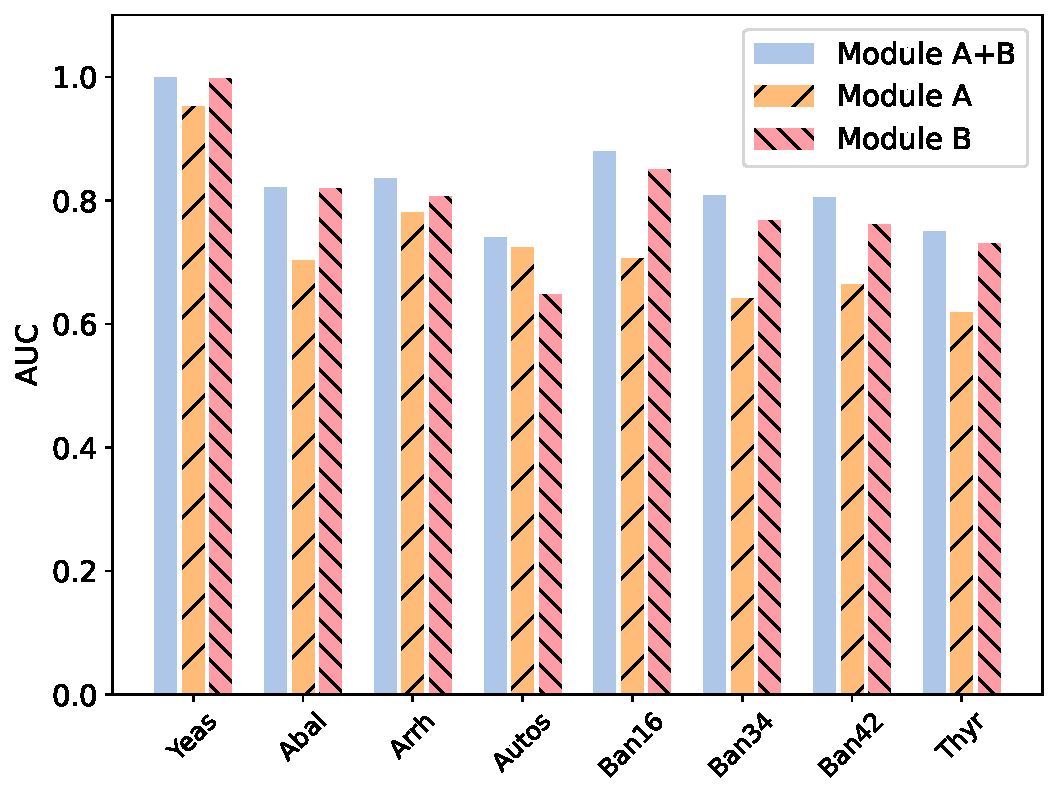
\includegraphics[width=0.45\textwidth,
trim=0.05cm 0.35cm 0.1cm 0.2cm,clip]{all_datasets_auc_values_8_16.pdf}}
    \caption{{Visual comparison of AUC performance across 16 datasets.}}
    \label{fig: Ablation experiments for various datasets}
\end{figure}

The experimental results reveal the following intrinsic characteristics regarding the mechanism of GBNAD.
% 揭示了算法的内在特点

\begin{enumerate}[\indent(1)]
    \item {Dominance of Local Force (Module B):} On the majority of datasets, such as {Card, Iris, Musk}, Module B outperforms Module A. The AUC of Module B is generally closer to that of the complete model. This suggests that for most anomaly detection tasks, local interaction information plays a primary role in distinguishing anomalies from normal samples.
    
    \item {Necessity of Global Structure (Module A):} Although Module A contributes less on average, it plays a critical role in specific datasets. Notably, on datasets like {Page} and {Pend}, Module A outperforms Module B. This indicates that these datasets likely contain anomalies defined by global topological isolation rather than local density variations. Module A effectively captures these global patterns, compensating for the limitations of the local force model.
    
    \item {Complementarity:} Module A offers a coarse-grained view based on global structure, while Module B provides a fine-grained view based on physical interactions. The consistent superiority of GBNAD demonstrates that fusing these two perspectives eliminates the bias of a single view, resulting in a robust detector capable of handling diverse anomaly types.
\end{enumerate}

Additionally, a key advantage of Module A is its high cost-effectiveness. As shown in Table \ref{Ablation_experiments_results}, Module A is computationally lightweight. For instance, in the {Thyr} dataset, Module A accounts for less than 2.3\% of the total runtime, yet incorporating it boosts the AUC from 0.73 to 0.75. This significant performance gain at a negligible computational cost confirms that Module A serves as an efficient global filter, while Module B acts as a precise local refiner.


\section{Conclusion and future work}
\label{Conclusion}
This work proposes an unsupervised anomaly detection algorithm named GBNAD. 
The algorithm introduces the innovative EGB model and integrates it with the ACF metric, establishing a physics-informed multi-granularity anomaly detection framework. 
By fusing two complementary modules, the local anomaly force metric and the global structure metric, GBNAD effectively evaluates anomaly degrees across multiple perspectives. 
This design addresses key challenges in existing physics-informed methods, including high computational complexity, sensitivity to outliers, and limited scalability, while preserving the inherent interpretability of the physical model.
Experimental evaluations on real-world datasets demonstrate the superior detection performance of the proposed method compared to state-of-the-art baselines. 

Moving forward, we plan to address current limitations by developing adaptive mechanisms for hyperparameter $k$ selection, generalizing the framework to accommodate categorical and mixed-type data, and designing incremental updating strategies to tackle concept drift in streaming data scenarios.

% In future work, we plan to address several limitations. First, we will explore adaptive mechanisms for automatically selecting the neighborhood parameter $k$, as its variation has a considerable impact on performance. 
% Second, while the current method focuses on numerical data, extending GBNAD to handle categorical or mixed-type datasets will further enhance its universality.
% {Finally, although GBNAD is designed for static environments, the adaptive nature of granular-balls holds substantial potential for handling streaming data and concept drift. We intend to investigate incremental granular-ball updating mechanisms to extend the framework to dynamic anomaly detection scenarios.}

\section*{Acknowledgments}

This work was supported by the National Natural Science Foundation of China (62306196) and Sichuan Science and Technology Program (2026NSFSC0783)



\bibliographystyle{elsarticle-num} %plainnat elsarticle-num elsarticle-harv elsarticle-num-names abbrv
\bibliography{myGBNADreference}
\end{document}

